\section{Case Study Results}\label{sec:case-study}
In this section, we report and discuss the results for each research question. {\color{blue}For each research question, we collect information about smell, fault hazard, and vulnerability codes of JavaScript files of the studied systems, and more specifically those which end with the \textsl{.js} extension. Also, we don't take in account the JavaScript files with \textsl{.min.js} extension, because they are a minified version of \textsl{.js} files that we already keep in our study. In this way, we avoid redundancy in our analyzes.}

\subsection*{(RQ1) Is the risk of fault higher in files with code smells in comparison with those without code smell?}

%\textbf{Motivation}. Code smells are poor solutions in software design and implementation problems. Previous studies such as Jaafar et al.~\cite{jaafar2013mining} has shown that the fault-proneness of modules are significantly different between implementations with code smells and implementations without them. As stated by ~\cite{jaafar2013mining}: ``classes having dependencies with anti-patterns are more fault-prone than others". However, their study has been done on Java software systems. To the best of our knowledge, less is known on the code smells of JavaScript. Hence, in this research question we aim to explore how code smells affect the reliability of a software developed in JavaScript.

%This knowledge helps software practitioners plan to detect the code smells as much early as possible in the very beginning phase of software development before the code base gets %bigger.%

\begin{figure*}[t]
\centering%
\subfigure[express.js]{%
{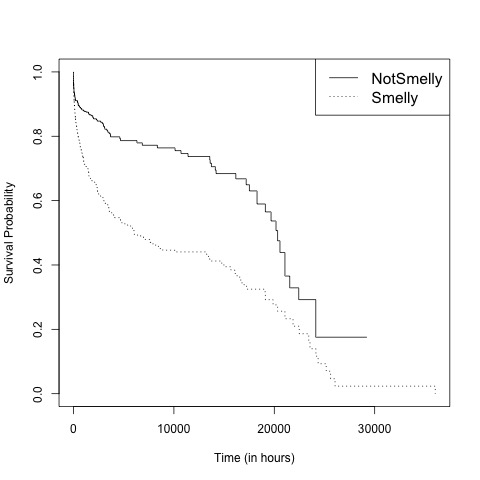
\epsfig{file = pdfs/Express_bugs_smells_file-grain_rplot.jpg, width = 3.5cm}}%
}
\subfigure[request.js]{%
{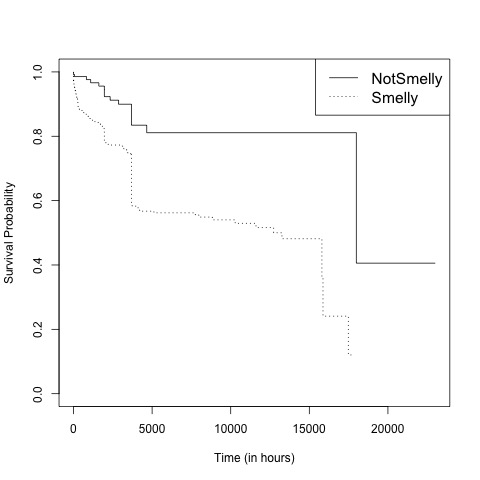
\epsfig{file = pdfs/Request_bugs_smells_file-grain_rplot.jpg, width = 3.5cm}}%
}
\subfigure[less.js]{%
{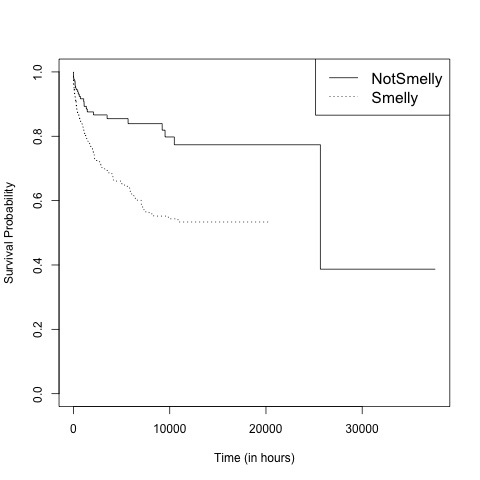
\epsfig{file = pdfs/Less_bugs_smells_file-grain_rplot.jpg, width = 3.5cm}}%
}
\subfigure[grunt.js]{%
{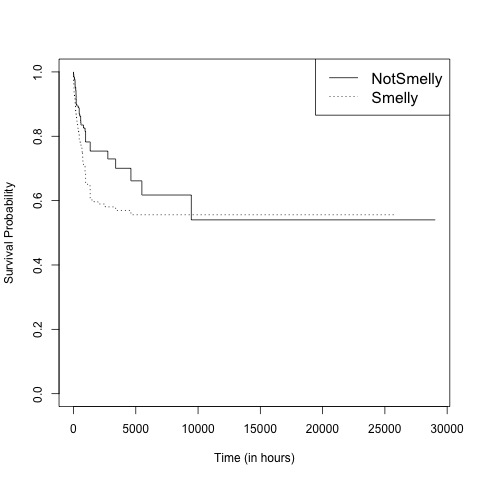
\epsfig{file = pdfs/Grunt_bugs_smells_file-grain_rplot.jpg, width = 3.5cm}}%
}
\subfigure[bower.js]{%
{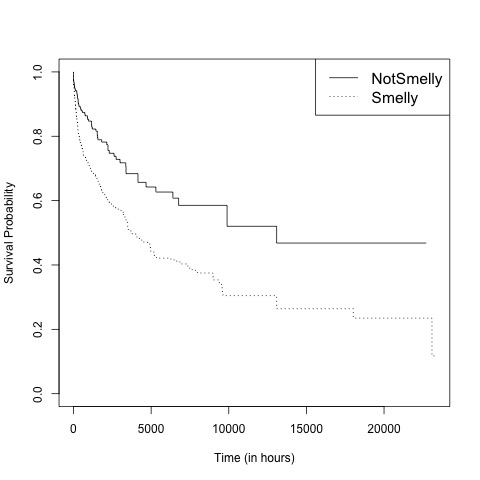
\epsfig{file = pdfs/Bower_bugs_smells_file-grain_rplot.jpg, width = 3.5cm}}%
}
\subfigure[jquery.js]{%
	{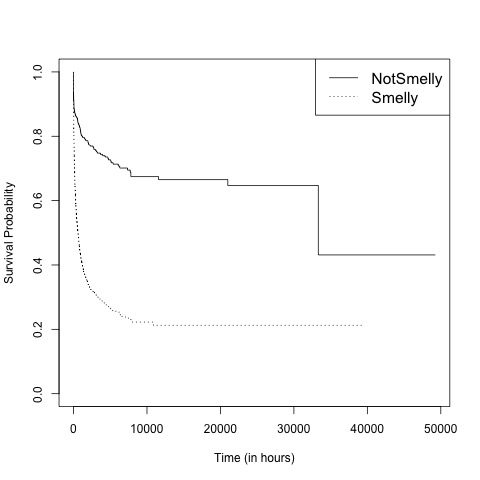
\epsfig{file = pdfs/Jquery_bugs_smells_file-grain_rplot.jpg, width = 3.5cm}}%
}
\subfigure[hexo.js]{%
	{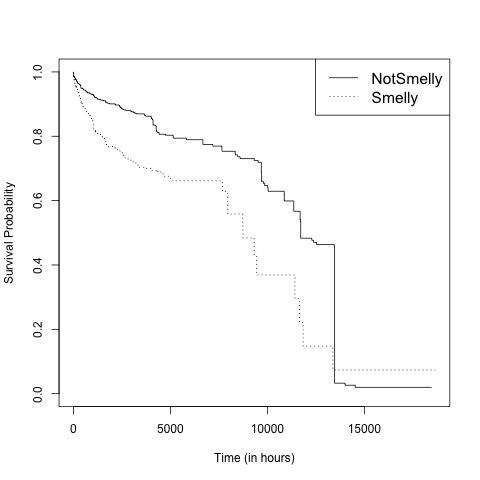
\epsfig{file = pdfs/Hexo_bugs_smells_file-grain_rplot.jpg, width = 3.5cm}}%
}
\subfigure[leaflet.js]{%
	{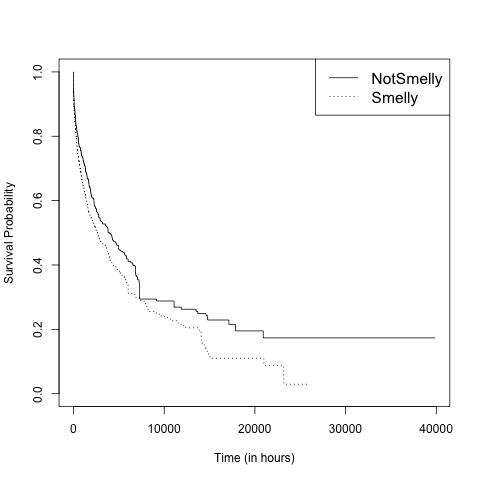
\epsfig{file = pdfs/Leaflet_bugs_smells_file-grain_rplot.jpg, width = 3.5cm}}%
}
\subfigure[ramda.js]{%
	{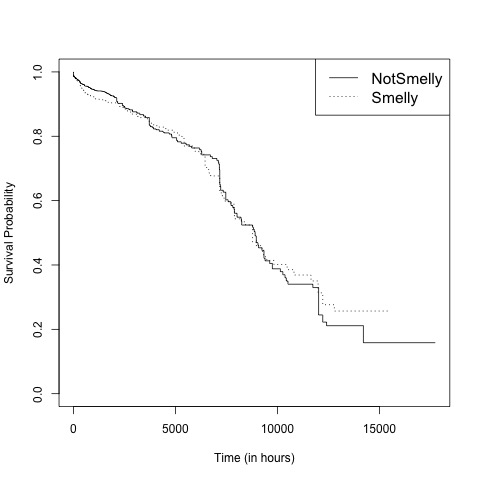
\epsfig{file = pdfs/Ramda_bugs_smells_file-grain_rplot.jpg, width = 3.5cm}}%
}
\subfigure[chart.js]{%
	{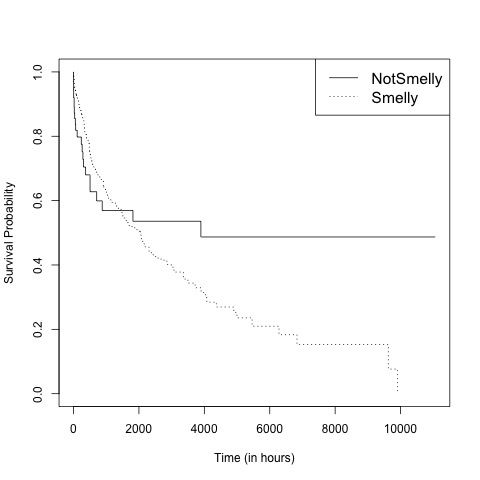
\epsfig{file = pdfs/Chart_bugs_smells_file-grain_rplot.jpg, width = 3.5cm}}%
}
\subfigure[riot.js]{%
	{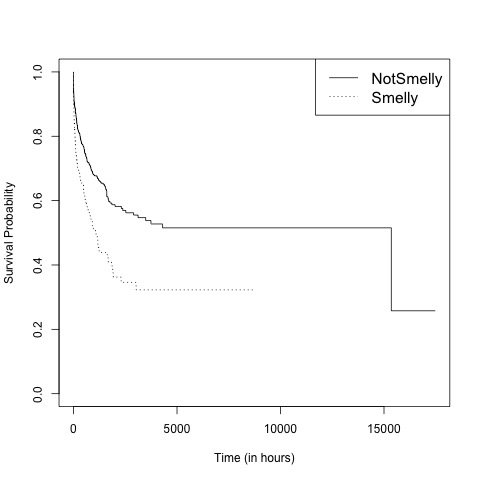
\epsfig{file = pdfs/Riot_bugs_smells_file-grain_rplot.jpg, width = 3.5cm}}%
}
\subfigure[vue.js]{%
	{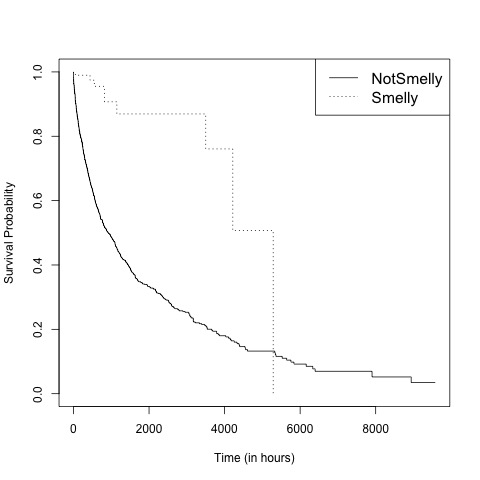
\epsfig{file = pdfs/Vue_bugs_smells_file-grain_rplot.jpg, width = 3.5cm}}%
}
\subfigure[moment.js]{%
	{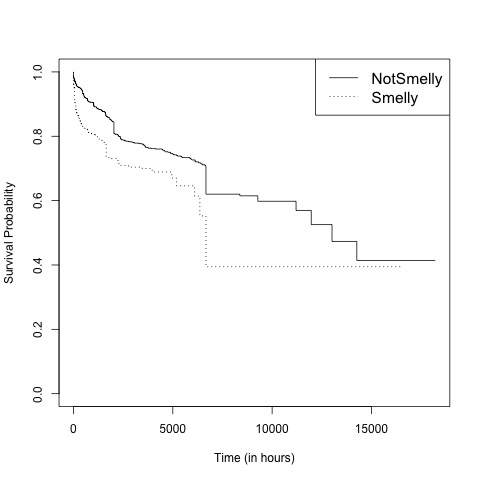
\epsfig{file = pdfs/Moment_bugs_smells_file-grain_rplot.jpg, width = 3.5cm}}%
}
\subfigure[webpack.js]{%
	{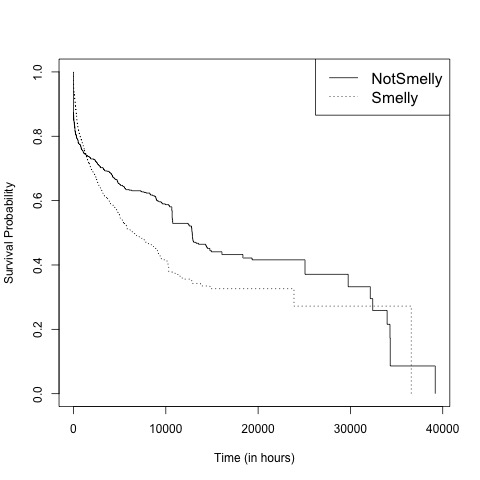
\epsfig{file = pdfs/Webpack_bugs_smells_file-grain_rplot.jpg, width = 3.5cm}}%
}
\subfigure[webtorrent.js]{%
	{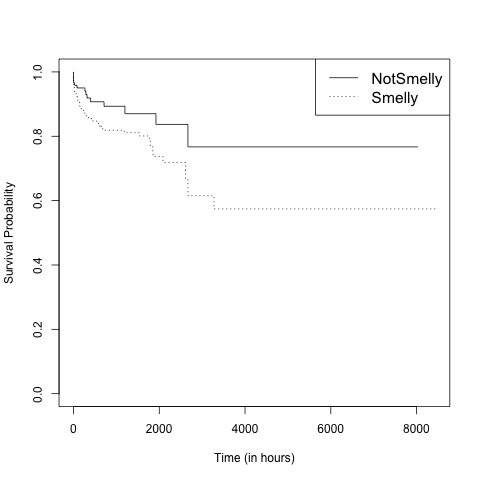
\epsfig{file = pdfs/Webtorrent_bugs_smells_file-grain_rplot.jpg, width = 3.5cm}}%
}
\caption{Survival probability trends of smelly codes vs. non-smelly codes in our fifteen JavaScript projects with the file grain approach (hazard study).\vspace{-10pt}}
\label{rq1}
\end{figure*}

\begin{table*}[t]
	\centering
	\scriptsize
	\caption{Fault hazard ratios for each project with the line grain approach. $exp(coef)$ values means higher hazard rates.}
	\label{hazardlinegrain}
	\begin{tabular}{l|l|l|l}
		\hline
		module & $exp(coef)$ & $p$-value (Cox hazard model) & $p$-value (Proportional hazards assumption)     \\ \hline
		express  & 1.341 & 0.002 & 0.192 \\ \hline
		request  & 2.538 & 0.028e-2 & 0.602 \\ \hline
		less  & 1.791 & 0.003 & 0.419 \\ \hline
		bower	 & 1.321 & 0.027 & 0.982 \\ \hline
		grunt    & 0.594 & 0.005 & 0.019 \\ \hline
		jquery	 & 3.436 & 0 & 1.197e-8 \\ \hline
		vue   & 0.062 & 0.011e-9 & 0.843 \\ \hline
		ramda 	 & 0.460 & 0.01e-8 & 3.691e-5 \\ \hline
		leaflet	 & 0.725 & 0.088e-4 & 0.739 \\ \hline
		hexo	 & 1.199 & 0.077 & 0.945 \\ \hline
		chart	 & 0.711 & 0.136 & 1.46e-9 \\ \hline
		webpack	 & 0.603 & 0 & 0 \\ \hline
		webtorrent & 1.222 & 0.047e-9 & 0.045 \\ \hline
		moment	 & 0.941 & 0.401 & 5.046e-5 \\ \hline
		riot	 & 1.047 & 0.586 & 0.797 \\ \hline
	\end{tabular}

\end{table*}

\begin{figure*}[t]
	\centering%
	\subfigure[express.js]{%
		{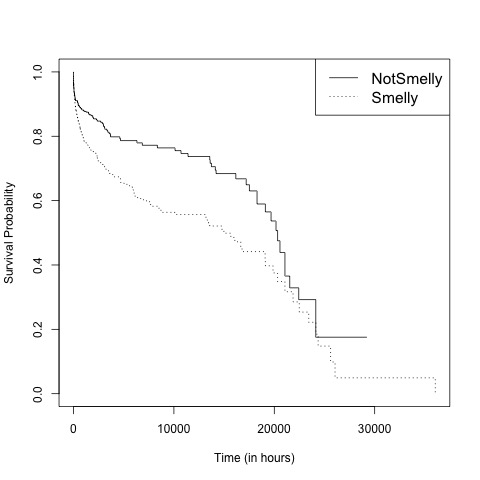
\epsfig{file = pdfs/Express_bugs_smells_line-grain_large_rplot.jpg, width = 3.5cm}}%
	}
	\subfigure[request.js]{%
		{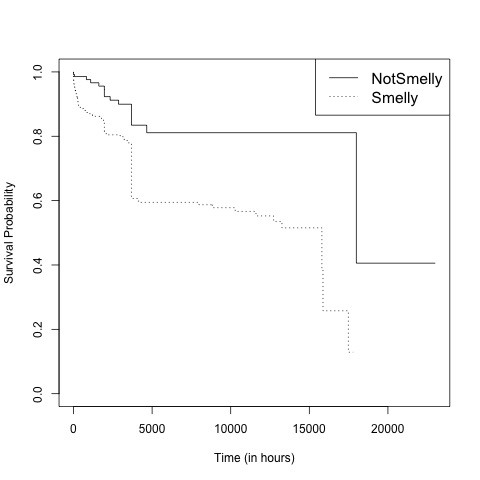
\epsfig{file = pdfs/Request_bugs_smells_line-grain_large_rplot.jpg, width = 3.5cm}}%
	}
	\subfigure[less.js]{%
		{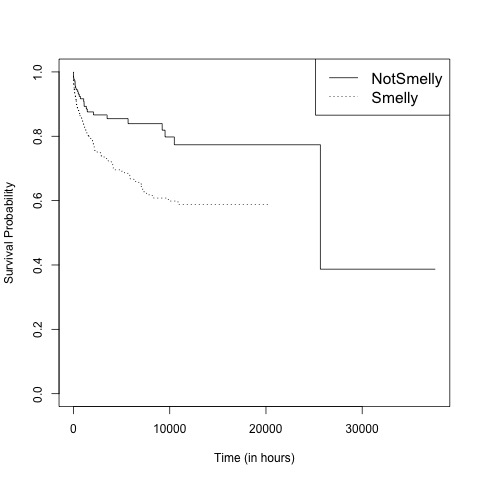
\epsfig{file = pdfs/Less_bugs_smells_line-grain_large_rplot.jpg, width = 3.5cm}}%
	}
	\subfigure[grunt.js]{%
		{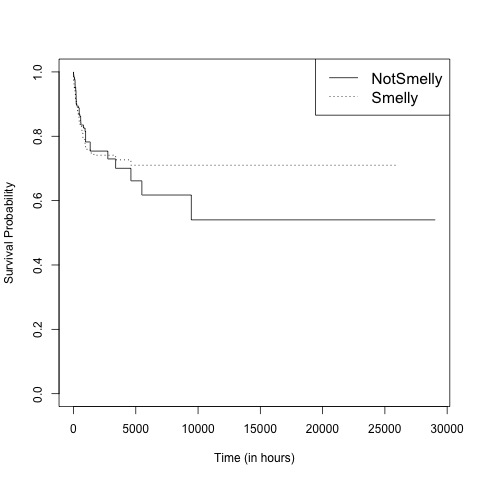
\epsfig{file = pdfs/Grunt_bugs_smells_line-grain_large_rplot.jpg, width = 3.5cm}}%
	}
	\subfigure[bower.js]{%
		{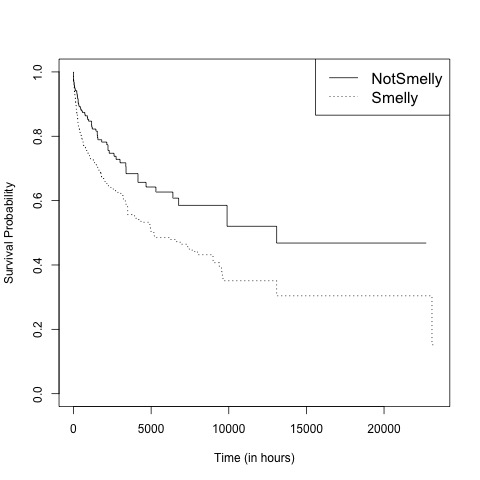
\epsfig{file = pdfs/Bower_bugs_smells_line-grain_large_rplot.jpg, width = 3.5cm}}%
	}
	\subfigure[jquery.js]{%
		{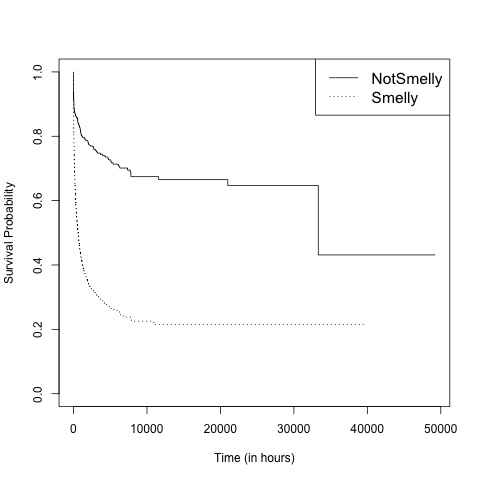
\epsfig{file = pdfs/Jquery_bugs_smells_line-grain_large_rplot.jpg, width = 3.5cm}}%
	}
	\subfigure[hexo.js]{%
		{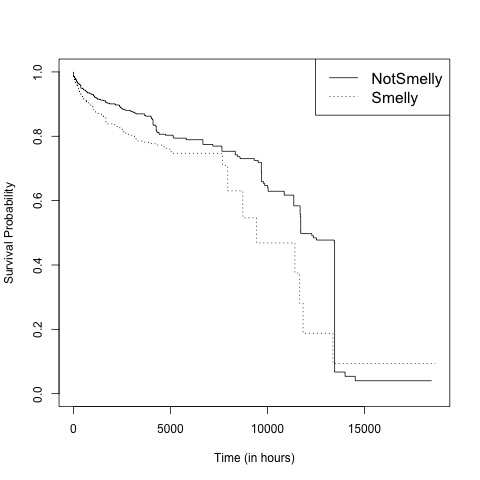
\epsfig{file = pdfs/Hexo_bugs_smells_line-grain_large_rplot.jpg, width = 3.5cm}}%
	}
	\subfigure[leaflet.js]{%
		{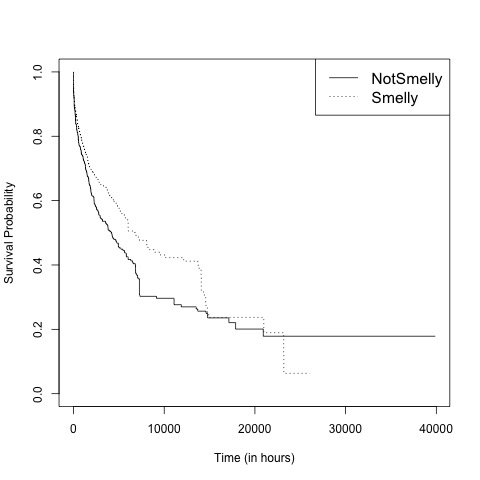
\epsfig{file = pdfs/Leaflet_bugs_smells_line-grain_large_rplot.jpg, width = 3.5cm}}%
	}
	\subfigure[ramda.js]{%
		{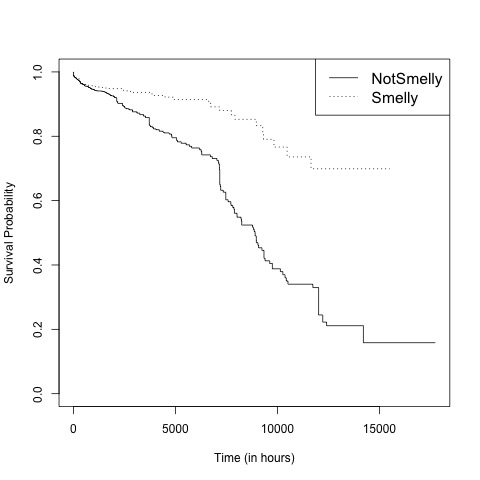
\epsfig{file = pdfs/Ramda_bugs_smells_line-grain_large_rplot.jpg, width = 3.5cm}}%
	}
	\subfigure[chart.js]{%
		{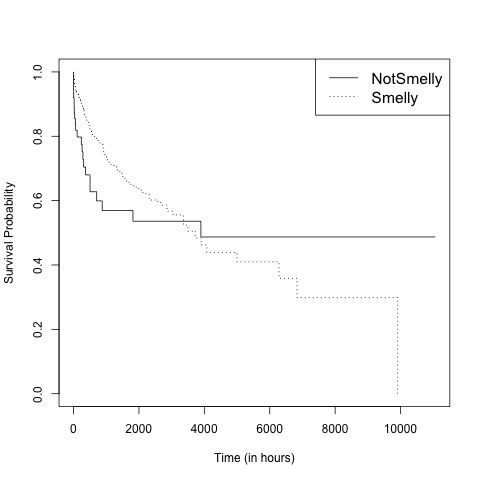
\epsfig{file = pdfs/Chart_bugs_smells_line-grain_large_rplot.jpg, width = 3.5cm}}%
	}
	\subfigure[riot.js]{%
		{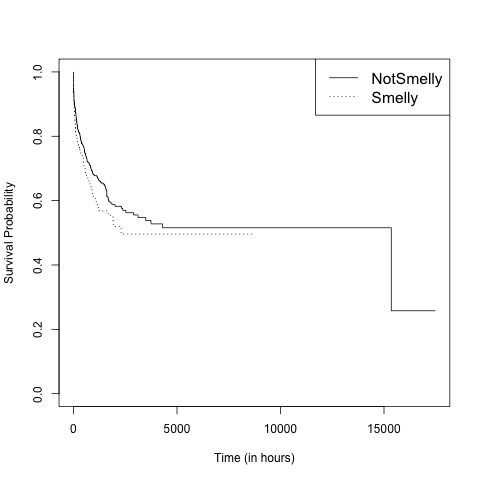
\epsfig{file = pdfs/Riot_bugs_smells_line-grain_large_rplot.jpg, width = 3.5cm}}%
	}
	\subfigure[vue.js]{%
		{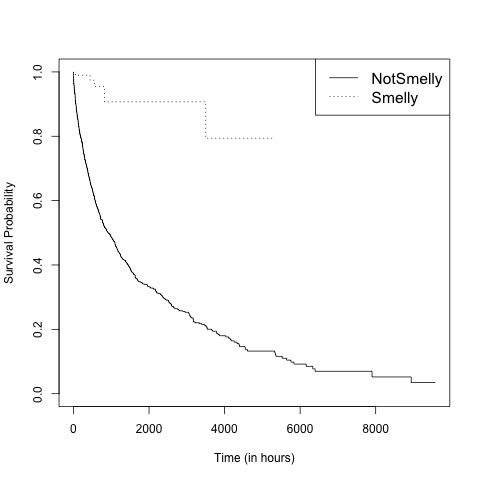
\epsfig{file = pdfs/Vue_bugs_smells_line-grain_large_rplot.jpg, width = 3.5cm}}%
	}
	\subfigure[moment.js]{%
		{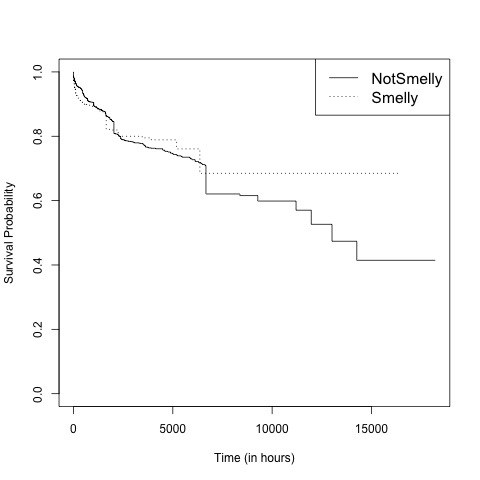
\epsfig{file = pdfs/Moment_bugs_smells_line-grain_large_rplot.jpg, width = 3.5cm}}%
	}
	\subfigure[webpack.js]{%
		{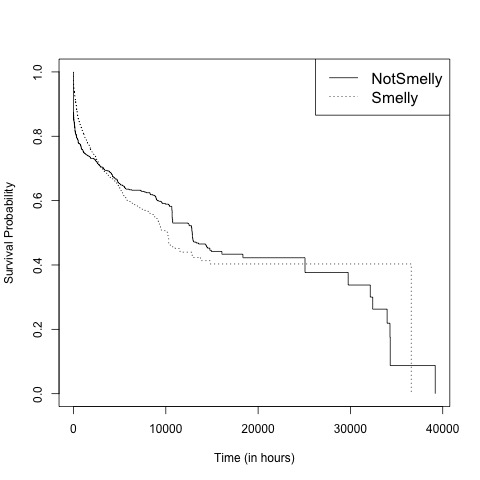
\epsfig{file = pdfs/Webpack_bugs_smells_line-grain_large_rplot.jpg, width = 3.5cm}}%
	}
	\subfigure[webtorrent.js]{%
		{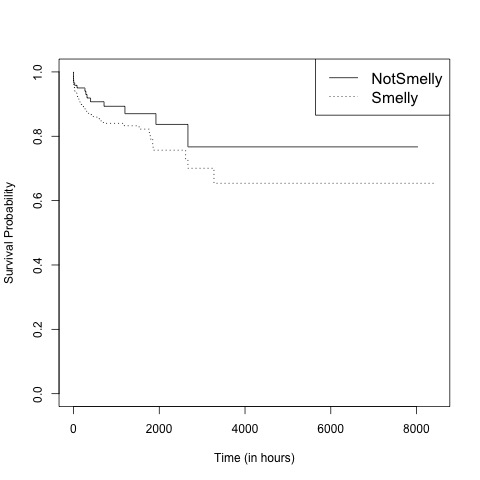
\epsfig{file = pdfs/Webtorrent_bugs_smells_line-grain_large_rplot.jpg, width = 3.5cm}}%
	}
	\caption{Survival probability trends of smelly codes vs. non-smelly codes in our fifteen JavaScript projects with the line grain including dependencies approach.\vspace{-10pt}}
	\label{rq1-2}
\end{figure*}

\textbf{Approach}. We use our framework described in Section~\ref{extraction} {\color{blue}(Figure~\ref{process})} to collect information about the occurrence of the 12 studied code smells in our {\color{blue}fifteen} subject systems. %fetch all the data considering all 12 types of code smells.
For each file and for each revision $r$ (\ie{} corresponding to a commit), we also compute the following metrics:
\begin{itemize}
\item \textbf{Time:} the number of hours between the previous revision of the file and the revision $r$. 
We set the time of the first revision to zero.
\item \textbf{Smelly:} this is our covariate of interest. It takes the value $1$ if the revision $r$ of the file contains a code smell and $0$ if it doesn't contain any of the 12 studied code smells. 
\item \textbf{Event:} {\color{blue}for the file grain approach,} this metric takes the value $1$ if the revision $r$ is a fault-fixing change and $0$ otherwise. We use the SZZ algorithm to insure that the file contained a code smell when the fault was introduced. {\color{blue}For the line grain and line grain including dependencies approaches, this metric takes the value $1$ if the revision $r$ is a fault-fixing change and if there is at least one match between the fault lines and the smell lines, and $0$ otherwise. Indeed, if there is no matching, we consider that the fault-fixing change doesn't fix any code smells.}
\end{itemize}

Using the smelly metric, we divide our dataset in two groups: one group containing files with code smells (\ie{} smelly = 1) and another group containing files without any of the 12 studied code smells (\ie{} smelly = 0). For each group we create an individual Cox hazard model. In each group, the covariate of interest (\ie{} smelly) is a constant function (with value either 1 or 0), hence, there is no need for a link function to establish a linear relationship between this covariate and our event of interest, \ie{} the occurrence of a fault. We use the \textsl{survfit} and \textsl{coxph} functions from R~\cite{rPackage} to analyze our Cox hazard models.

In addition to building Cox hazard models, we test the following null hypothesis: \emph{$H^{1}_{0}$: There is no difference between the probability of a fault occurrence in a file containing code smells and a file without code smells}. We use the \textsl{log-rank} test (which compares the survival distributions of two samples), to accept or refute this null hypothesis.

\textbf{Findings}. {\color{blue}File grain} results presented in Figure~\ref{rq1} show that files containing code smells experience faults faster than files without code smells. {\color{blue}Table~\ref{hazardlinegrain} (line grain results) and Figure~\ref{rq1-2} (line grain including dependencies results) show the same minimized but still acceptable observation, wich means files containing code smells experience faults faster than files without code smells.} The $Y$-axis in Figure~\ref{rq1} {\color{blue}and Figure~\ref{rq1-2}} represents the probability of a file \emph{surviving} a fault occurrence. Hence a low value on the $Y$-axis means a low \emph{survival} rate (\ie{} a high hazard or high risk of fault occurrence).  
For all {\color{blue}fifteen} projects, {\color{blue}and for each approach (file grain, line grain, and line grain including dependencies),} we calculated relative hazard rates (using Equation~\ref{eq3} from Section~\ref{survival}) between files containing code smells and files without code smells. Results show that, on average, files without code smells have hazard rates {\color{blue}76\% lower than files with code smells in our file grain analysis, 20\% lower in our line grain analysis, and 38\% lower in our line grain analysis including dependencies. It is normal to see this pourcentage decreasing in line grain approach, because we add an additional matching condition to set the \emph{event} to $1$. Between the line grain and the line grain including dependencies analyzes, this pourcentage increases due to the increasing of the fault lines number considering during the compute of \emph{event}.} We performed a \textsl{log-rank} test comparing the survival distributions of files containing code smells and files without any of the studied code smells and obtained $p$-values lower than $0.05$ for {\color{blue}most of the fifteen} studied systems. Hence, we reject $H^{1}_{0}$.
Since our detection of code smells depends on our selected threshold value (\ie{} the top 10\% value chosen in Section~\ref{extraction}), we conducted a sensitivity analysis to assess the potential impact of this threshold selection on our result. More specifically, we rerun all our analysis with threshold values at top 20\% and top 30\%. We observed no significant differences in the results. Hence, we conclude that:

\hypobox{JavaScript files without code smells have hazard rates {\color{blue}76\%} lower than JavaScript files with code smells {\color{blue}in the file grain approach}, and this difference is statistically significant. {\color{blue}Plus, this difference still remains significant in the line grain including dependencies approach, because hazard rates reach 38\%.}}


\begin{figure}[t]
\centering
\captionsetup{font=small}
\minipage{0.2\textwidth}
  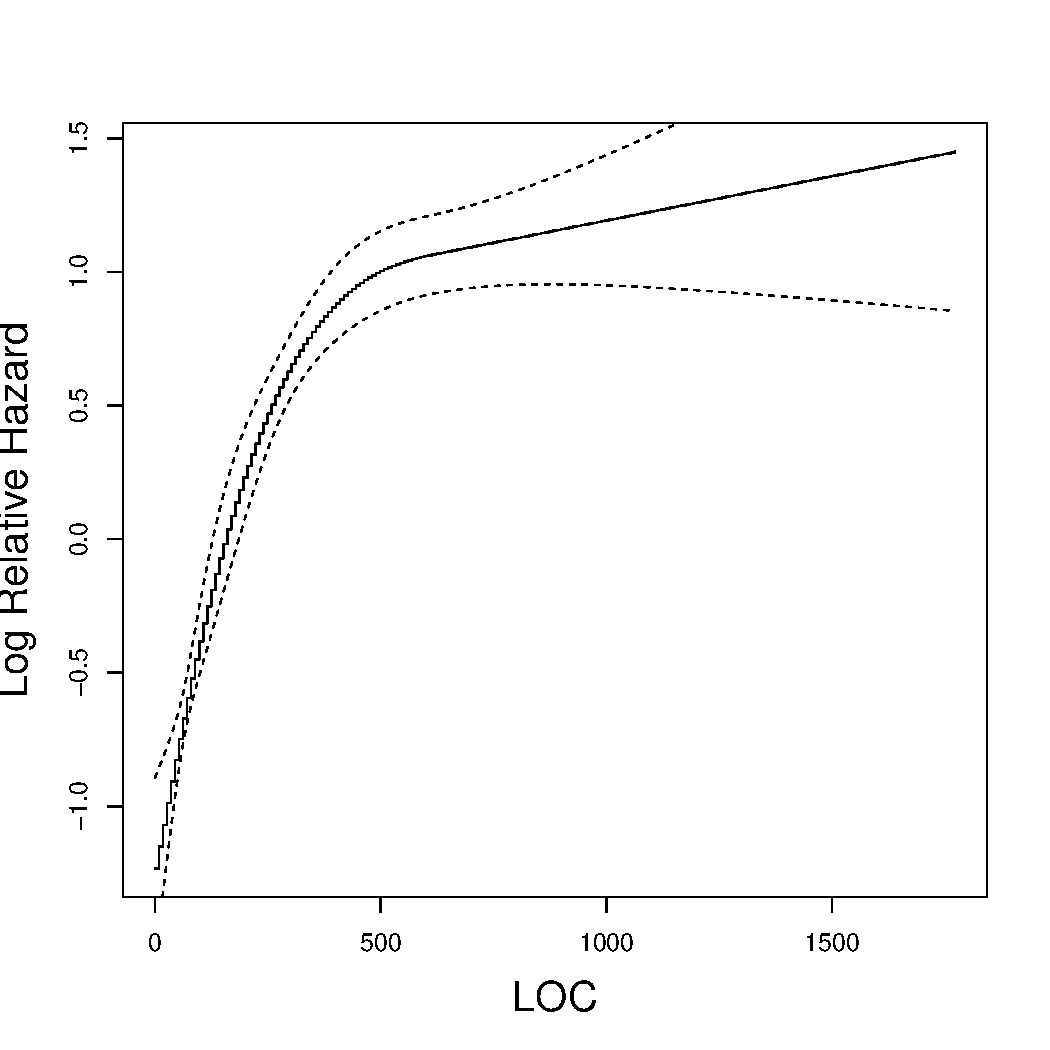
\includegraphics[width=\linewidth]{pdfs/linkExpress.pdf}
\endminipage
\minipage{0.2\textwidth}
  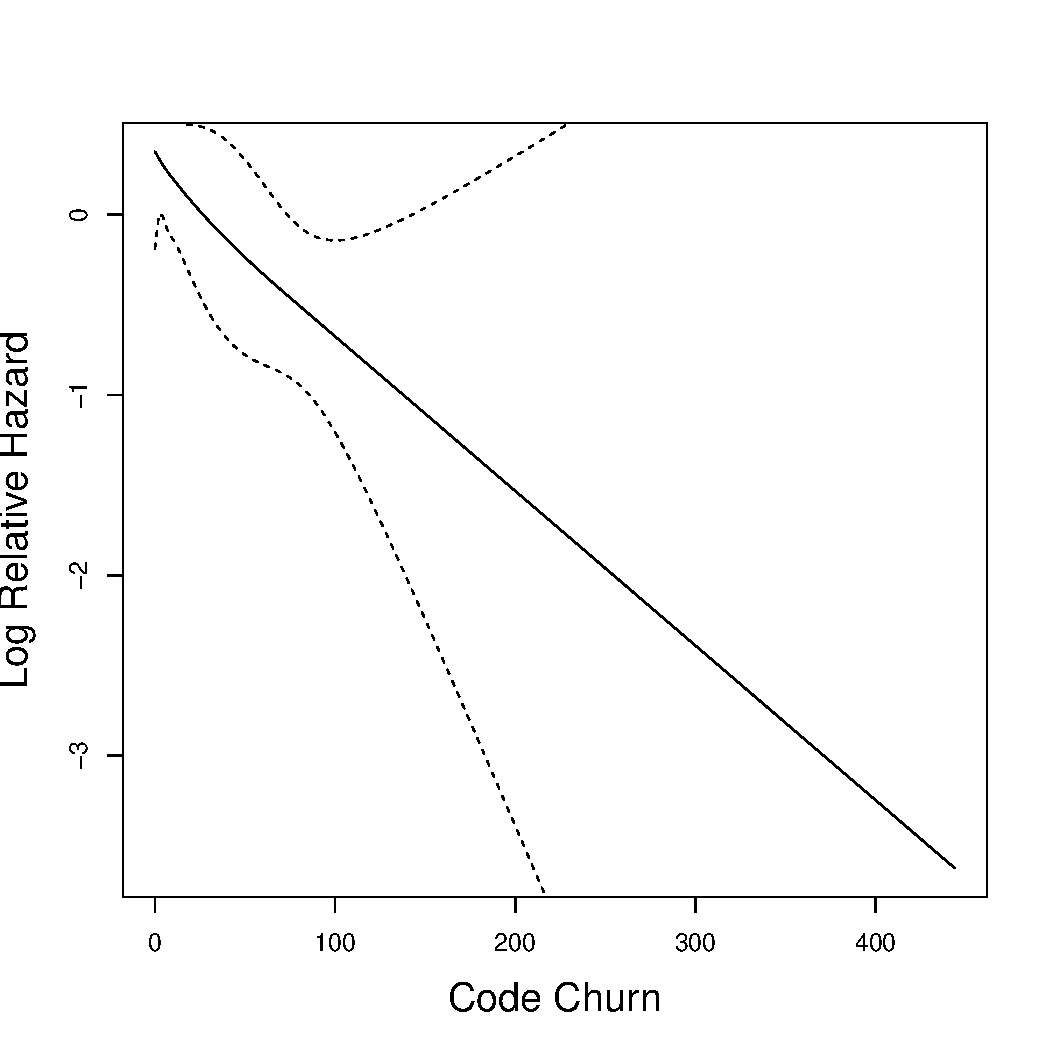
\includegraphics[width=\linewidth]{pdfs/linkTotalChurnGrunt.pdf}
\endminipage
\caption{Determining a link function for express.js (left figure) and grunt.js (right figure) modules for two covariates: LOC and Code Churn respectively.\vspace{-10pt}}\label{link}
\end{figure}

\subsection*{(RQ2) Are JavaScript files with code smells equally fault-prone?}

%\begin{table*}[t]
%\centering%
%\caption{Covariates coeffiecients on the defects. Higher exp(coef) means higher hazard rate.}
%\begin{tabular}{c|c|c|c|c|c|c}
%\hline
%module & covariate & exp(coef) & se(coef) & z & p & Non-proportionality test (p-value) \\ \hline
%\multirow{3}{*}{express} & No.Previous-Bugs & 1.01842956 & 0.00300334 & 6.08 & 0.0000000012 & 0.887 \\ \cline{2-7}
% & cond.assign & 1.55093782 & 0.14811000 & 2.96 & 0.0030 & 0.561 \\ \cline{2-7}
% & LOC & 1.00111187 & 0.00019567 & 5.68 & 0.0000000135 & 0.382 \\ \hline
%\multirow{2}{*}{grunt} & cond.assign & 2.36768081 & 0.24248431 & 3.55 & 0.00038 & 0.2237 \\ \cline{2-7}
% & nested.callbacks & 3.13565940 & 0.41026000 & 2.79 & 0.00534 & 0.8147 \\ \hline
%\multirow{3}{*}{bower} & No.Previous-Bugs & 1.025646 & 0.007863 & 3.22 & 0.0013 & 0.415 \\ \cline{2-7}
% & max.depth & 9.222632 & 0.452966 & 4.90 & 0.00000094 & 0.960 \\ \cline{2-7}
% & LOC & 1.000643 & 0.000295 & 2.18 & 0.0295 & 0.414 \\ \hline
%\multirow{3}{*}{less} & No.Previous-Bugs & 1.036634202 & 0.003126697 & 11.51 & 0.000002 & 0.739 \\ \cline{2-7}
% & complex.switch.case & 0.484588521 & 0.332039480 & -2.18 & 0.02912 & 0.4177 \\ \cline{2-7}
% & cond.assign & 1.664212015 & 0.131560216 & 3.87 & 0.00011 & 0.9154 \\ \hline
%\multirow{3}{*}{request} & No.Previous-Bugs & 1.0675617 & 0.0218429 & 2.99 & 0.0028 & 0.4074 \\ \cline{2-7}
% & max.depth & 0.1723391 & 0.4346634 & -4.05 & 0.000052 & 0.6207 \\ \cline{2-7}
% & LOC & 1.0009179 & 0.0003798 & 2.42 & 0.0157 & 0.8668 \\ \hline
%\end{tabular}
%\end{table*}

% Please add the following required packages to your document preamble:
% \usepackage{multirow}
%\begin{table*}[t]
%\centering%
%\caption{Covariates coeffiecients on the defects. Higher exp(coef) means higher hazard rate.}
%\begin{tabular}{c|c|c|c|c}
%\hline
%module & covariate & exp(coef) & p & Non-proportionality test (p-value) \\ \hline
%\multirow{3}{*}{express} & No.Previous-Bugs & 1.01842956 & 0.0000000012 & 0.887 \\ \cline{2-5}
% & cond.assign & 1.55093782 & 0.0030 & 0.561 \\ \cline{2-5}
% & LOC & 1.00111187 & 0.0000000135 & 0.382 \\ \hline
%\multirow{2}{*}{grunt} & cond.assign & 2.36768081 & 0.00038 & 0.2237 \\ \cline{2-5}
% & nested.callbacks & 3.13565940 & 0.00534 & 0.8147 \\ \hline
%\multirow{3}{*}{bower} & No.Previous-Bugs & 1.025646 & 0.0013 & 0.415 \\ \cline{2-5}
% & max.depth & 9.222632 & 0.00000094 & 0.960 \\ \cline{2-5}
% & LOC & 1.000643 & 0.0295 & 0.414 \\ \hline
%\multirow{3}{*}{less} & No.Previous-Bugs & 1.036634202 & 0.000002 & 0.739 \\ \cline{2-5}
% & complex.switch.case & 0.484588521 & 0.02912 & 0.4177 \\ \cline{2-5}
% & cond.assign & 1.664212015 & 0.00011 & 0.9154 \\ \hline
%\multirow{3}{*}{request} & No.Previous-Bugs & 1.0675617 & 0.0028 & 0.4074 \\ \cline{2-5}
% & max.depth & 0.1723391 & 0.000052 & 0.6207 \\ \cline{2-5}
% & LOC & 1.0009179 & 0.0157 & 0.8668 \\ \hline
%\end{tabular}
%\end{table*}

% Please add the following required packages to your document preamble:
% \usepackage{multirow}
\begin{table}[t]
\centering
\scriptsize
\caption{Hazard ratios for each type of code smells with file grain approach. Higher $exp(coef)$ values means higher hazard rates.}
\begin{tabular}{c|c|c|p{1.1cm}|p{1.3cm}}
\hline
module & covariate & $exp(coef)$ & $p$-value (Cox hazard model) & $p$-value (Proportional hazards assumption) \\ \hline
\multirow{4}{*}{express}
 & No.Previous-Bugs & 1.031 & 0 & 0.076 \\ \cline{2-5}
 & Long Methods & 3.363 & 0.012e-11 & 0.14 \\ \cline{2-5}
 & Complex Switch Case & 2.528 & 0.043e-8 & 0.322 \\ \cline{2-5}
 & Variable Re-assign & 1.927 & 0.056e-14 & 0.725  \\ \hline
\multirow{4}{*}{grunt} 
 & No.Previous-Bugs & 1.051 & 0.003 & 0.925 \\ \cline{2-5}
 & Nested Callbacks & 3.609 & 0.086e-3 & 0.65 \\ \cline{2-5}
 & Assign. in Cond. State. & 2.008 & 0.004 & 0.707 \\ \cline{2-5}
 & Long Methods & 1.8 & 0.019 & 0.098 \\ \hline
\multirow{5}{*}{bower}
 & No.Previous-Bugs & 1.047 & 0 & 0.596 \\ \cline{2-5}
 & LOC & 1.001 & 0.023e-13 & 0.379 \\ \cline{2-5}
 & Complex Code & 5.778 & 0 & 0.432 \\ \cline{2-5}
 & Long Methods & 3.55 & 0 & 0.525 \\ \cline{2-5}
 & Extra Bind & 3.03 & 0.097e-5 & 0.378 \\ \hline
\multirow{4}{*}{less}
 & No.Previous-Bugs & 1.024 & 0 & 0.313 \\ \cline{2-5}
 & Depth & 2.36 & 0.013e-2 & 0.95 \\ \cline{2-5}
 & Assign. in Cond. State. & 2.25 & 0.012e-10 & 0.169 \\ \cline{2-5}
 & Lengthy Lines & 2.07 & 0.027e-4 & 0.709 \\ \hline
\multirow{5}{*}{request}
 & No.Previous-Bugs & 1.053 & 0.097e-13 & 0.23 \\ \cline{2-5}
 & LOC & 1.001 & 0.022e-14 & 0.718 \\ \cline{2-5}
 & This Assign & 3.094 & 0.027e-12 & 0.4 \\ \cline{2-5}
 & Variable Re-assign & 2.614 & 0.063e-4 & 0.78 \\ \cline{2-5}
 & Complex Switch Case & 2.608 & 0.002 & 0.632 \\ \hline
\multirow{4}{*}{jquery}
 & LOC & 1.0001 & 0 & 0.164 \\ \cline{2-5}
 & Lengthy Lines & 2.025 & 0 & 0.393 \\ \cline{2-5}
 & Assign. in Cond. State. & 1.881 & 0.014e-6 & 0.123 \\ \cline{2-5}
 & Complex Code & 1.706 & 0 & 0.169 \\ \hline
\multirow{5}{*}{hexo}
 & No.Previous-Bugs & 1.255 & 0 & 0.355 \\ \cline{2-5}
 & LOC & 1.001 & 0 & 0.236 \\ \cline{2-5}
 & Chaine Methods & 2.511 & 0.044e-8 & 0.805 \\ \cline{2-5}
 & Variable Re-assign & 1.916 & 0.027e-11 & 0.523 \\ \cline{2-5}
 & Nested Callbacks & 1.915 & 0.02e-3 & 0.942 \\ \hline
\multirow{3}{*}{leaflet}
 & LOC & 1.0001 & 0.016e-10 & 0.14 \\ \cline{2-5}
 & Nested Callbacks & 1.494 & 0.009 & 0.373 \\ \cline{2-5}
 & Variable Re-assign & 1.24 & 0.082e-2 & 0.321 \\ \hline
\multirow{4}{*}{ramda}
 & LOC & 1.0001 & 0.033 & 0.122 \\ \cline{2-5}
 & Complex Switch Case & 3.64 & 0.034e-7 & 0.952 \\ \cline{2-5}
 & Long Parameter List & 3.487 & 0.011e-7 & 0.616 \\ \cline{2-5}
 & Complex Code & 2.859 & 0.076e-5 & 0.291 \\ \hline
\multirow{2}{*}{riot}
 & Variable Re-assign & 1.782 & 0.024e-12 & 0.09 \\ \cline{2-5}
 & This Assign & 1.445 & 0.002 & 0.458 \\ \hline
\multirow{2}{*}{vue}
 & Assign. in Cond. State. & 0.161 & 0.01 & 0.856 \\ \cline{2-5}
 & Variable Re-assign & 0.092 & 0.018e-19 & 0.149 \\ \hline
\multirow{4}{*}{moment}
 & No.Previous-Bugs & 1.014 & 0 & 0.326 \\ \cline{2-5}
 & Complex Switch Case & 9.495 & 0 & 0.914 \\ \cline{2-5}
 & Chained Methods & 4.148 & 0 & 0.119 \\ \cline{2-5}
 & This Assign & 2.925 & 0 & 0.327 \\ \hline
\multirow{4}{*}{webtorrent}
 & No.Previous-Bugs & 1.063 & 0.014e-9 & 0.053 \\ \cline{2-5}
 & LOC & 1.001 & 0.014e-6 & 0.053 \\ \cline{2-5}
 & This Assign & 1.967 & 0.019e-2 & 0.28 \\ \cline{2-5}
 & Variable Re-assign & 1.883 & 0.01 & 0.399 \\ \hline
\end{tabular}
\label{smelltypes}
\vspace{-15pt}
\end{table}

\begin{table}[t]
	\centering
	\scriptsize
	\caption{Hazard ratios for each type of code smells with line grain approach. Higher $exp(coef)$ values means higher hazard rates.}
	\begin{tabular}{c|c|c|p{1.1cm}|p{1.3cm}}
		\hline
		module & covariate & $exp(coef)$ & $p$-value (Cox hazard model) & $p$-value (Proportional hazards assumption) \\ \hline
		\multirow{2}{*}{express}
		& No.Previous-Bugs & 1.034 & 0 & 0.126 \\ \cline{2-5}
		& Variable Re-assign & 1.22 & 0.024 & 0.814  \\ \hline
		\multirow{4}{*}{grunt} 
		& No.Previous-Bugs & 1.064 & 0.009 & 0.693 \\ \cline{2-5}
		& Assign. in Cond. State. & 0.315 & 0.047 & 0.628 \\ \cline{2-5}
		& Chained Methods & 0.206 & 0.002 & 0.94 \\ \cline{2-5}
		& Lengthy Lines & 0.154 & 0.036e-3 & 0.053 \\ \hline
		\multirow{4}{*}{bower}
		& No.Previous-Bugs & 1.051 & 0 & 0.679 \\ \cline{2-5}
		& LOC & 1.001 & 0.064e-11 & 0.480 \\ \cline{2-5}
		& Variable Re-assign & 1.335 & 0.02 & 0.832 \\ \cline{2-5}
		& This Assign & 0.394 & 0.012e-5 & 0.998 \\ \hline
		\multirow{3}{*}{less}
		& No.Previous-Bugs & 1.024 & 0 & 0.566 \\ \cline{2-5}
		& Variable Re-assign & 1.446 & 0.033 & 0.652 \\ \cline{2-5}
		& Assign. in Cond. State. & 1.342 & 0.036 & 0.052 \\ \hline
		\multirow{3}{*}{request}
		& No.Previous-Bugs & 1.061 & 0.013e-13 & 0.185 \\ \cline{2-5}
		& LOC & 1.001 & 0 & 0.517 \\ \cline{2-5}
		& Variable Re-assign & 1.913 & 0.003 & 0.455 \\ \hline
		\multirow{4}{*}{jquery}
		& LOC & 1.0001 & 0 & 0.164 \\ \cline{2-5}
		& Lengthy Lines & 2.002 & 0 & 0.385 \\ \cline{2-5}
		& Assign. in Cond. State. & 1.881 & 0.014e-6 & 0.123 \\ \cline{2-5}
		& Complex Code & 1.684 & 0 & 0.164 \\ \hline
		\multirow{2}{*}{hexo}
		& No.Previous-Bugs & 1.25 & 0 & 0.296 \\ \cline{2-5}
		& LOC & 1.001 & 0.015e-8 & 0.251 \\ \hline
		\multirow{5}{*}{leaflet}
		& No.Previous-Bugs & 1.016 & 0 & 0.08 \\ \cline{2-5}
		& LOC & 1.0001 & 0.01e-2 & 0.192 \\ \cline{2-5}
		& Variable Re-assign & 0.712 & 0.025e-4 & 0.578 \\ \cline{2-5}
		& Complex Code & 0.485 & 0.003 & 0.179 \\ \cline{2-5}
		& Chained Methods & 0.405 & 0.034e-4 & 0.201 \\ \hline
		\multirow{4}{*}{ramda}
		& LOC & 1.0001 & 0.037 & 0.225 \\ \cline{2-5}
		& Nested Callbacks & 0.399 & 0.014e-2 & 0.271 \\ \cline{2-5}
		& Complex Code & 0.242 & 0.046 & 0.322 \\ \cline{2-5}
		& Chained Methods & 0.231 & 0.038 & 0.996 \\ \hline
		\multirow{4}{*}{chart}
		& No.Previous-Bugs & 1.151 & 0 & 0.113 \\ \cline{2-5}
		& Nested Callbacks & 0.321 & 0.034e-7 & 0.747 \\ \cline{2-5}
		& This Assign & 0.265 & 0 & 0.198 \\ \cline{2-5}
		& Long Parameter List & 0.191 & 0.036e-4 & 0.306 \\ \hline
		\multirow{2}{*}{riot}
		& This Assign & 0.125 & 0.047e-6 & 0.8 \\ \cline{2-5}
		& Long Parameter List & 0.105 & 0.069e-4 & 0.277 \\ \hline
		\multirow{2}{*}{vue}
		& Variable Re-assign & 0.069 & 0.065e-9 & 0.678 \\ \cline{2-5}
		& This Assign & 0.017 & 0.049e-3 & 0.156 \\ \hline
		\multirow{2}{*}{moment}
		& No.Previous-Bugs & 1.015 & 0 & 0.496 \\ \cline{2-5}
		& Long Methods & 0.261 & 0.003 & 0.425 \\ \hline
		\multirow{1}{*}{webpack}
		& Extra Bind & 0.295 & 0.035 & 0.969 \\ \hline
		\multirow{3}{*}{webtorrent}
		& No.Previous-Bugs & 1.054 & 0.075e-5 & 0.058 \\ \cline{2-5}
		& LOC & 1.001 & 0.018e-2 & 0.095 \\ \cline{2-5}
		& Nested Callbacks & 0.17 & 0.013 & 0.405 \\ \hline
	\end{tabular}
	\label{smelltypes2}
	\vspace{-15pt}
\end{table}

\begin{table}[t]
	\centering
	\scriptsize
	\caption{Hazard ratios for each type of code smells with line grain including dependencies approach. Higher $exp(coef)$ values means higher hazard rates.}
	\begin{tabular}{c|c|c|p{1.1cm}|p{1.3cm}}
		\hline
		module & covariate & $exp(coef)$ & $p$-value (Cox hazard model) & $p$-value (Proportional hazards assumption) \\ \hline
		\multirow{4}{*}{express}
		& No.Previous-Bugs & 1.034 & 0 & 0.124 \\ \cline{2-5}
		& Complex Code & 1.955 & 0.03e-2 & 0.152 \\ \cline{2-5}
		& Long Methods & 1.674 & 0.024 & 0.227 \\ \cline{2-5}
		& Variable Re-assign & 1.354 & 0.042e-2 & 0.742 \\ \hline
		\multirow{2}{*}{grunt} 
		& No.Previous-Bugs & 1.072 & 0.035e-2 & 0.495 \\ \cline{2-5}
		& Lengthy Lines & 0.402 & 0.001 & 0.288 \\ \hline
		\multirow{4}{*}{bower}
		& No.Previous-Bugs & 1.05 & 0 & 0.855 \\ \cline{2-5}
		& LOC & 1.001 & 0.07e-11 & 0.652 \\ \cline{2-5}
		& Complex Code & 2.314 & 0.006 & 0.734 \\ \cline{2-5}
		& Variable Re-assign & 1.579 & 0.019e-2 & 0.601 \\ \hline
		\multirow{2}{*}{less}
		& No.Previous-Bugs & 1.023 & 0 & 0.522 \\ \cline{2-5}
		& Variable Re-assign & 1.616 & 0.005 & 0.463 \\ \hline
		\multirow{3}{*}{request}
		& No.Previous-Bugs & 1.056 & 0.038e-13 & 0.188 \\ \cline{2-5}
		& LOC & 1.001 & 0.022e-14 & 0.664 \\ \cline{2-5}
		& Variable Re-assign & 2.316 & 0.089e-3 & 0.66 \\ \hline
		\multirow{4}{*}{jquery}
		& LOC & 1.0001 & 0 & 0.161 \\ \cline{2-5}
		& Lengthy Lines & 2.002 & 0 & 0.385 \\ \cline{2-5}
		& Assign. in Cond. State. & 1.881 & 0.014e-6 & 0.123 \\ \cline{2-5}
		& Complex Code & 1.684 & 0 & 0.164 \\ \hline
		\multirow{3}{*}{hexo}
		& No.Previous-Bugs & 1.254 & 0 & 0.325 \\ \cline{2-5}
		& LOC & 1.001 & 0.019e-11 & 0.269 \\ \cline{2-5}
		& Variable Re-assign & 1.321 & 0.004 & 0.896 \\ \hline
		\multirow{4}{*}{leaflet}
		& LOC & 1.0001 & 0.081e-10 & 0.101 \\ \cline{2-5}
		& Variable Re-assign & 0.755 & 0.047e-3 & 0.435 \\ \cline{2-5}
		& Complex Code & 0.485 & 0.003 & 0.179 \\ \cline{2-5}
		& Chained Methods & 0.434 & 0.091e-4 & 0.222 \\ \hline
		\multirow{3}{*}{ramda}
		& LOC & 1.0001 & 0.037 & 0.228 \\ \cline{2-5}
		& Nested Callbacks & 0.579 & 0.007 & 0.978 \\ \cline{2-5}
		& Complex Code & 0.242 & 0.046 & 0.322 \\ \hline
		\multirow{4}{*}{chart}
		& No.Previous-Bugs & 1.15 & 0 & 0.122 \\ \cline{2-5}
		& Nested Callbacks & 0.321 & 0.034e-7 & 0.747 \\ \cline{2-5}
		& This Assign & 0.281 & 0 & 0.173 \\ \cline{2-5}
		& Long Parameter List & 0.191 & 0.036e-4 & 0.306 \\ \hline
		\multirow{3}{*}{riot}
		& Variable Re-assign & 1.26 & 0.004 & 0.258 \\ \cline{2-5}
		& Chained Methods & 0.22 & 0.067e-3 & 0.602 \\ \cline{2-5}
		& This Assign & 0.125 & 0.046e-6 & 0.93 \\ \hline
		\multirow{2}{*}{vue}
		& Variable Re-assign & 0.092 & 0.018e-9 & 0.149 \\ \cline{2-5}
		& Depth & 0.033 & 0.066e-2 & 0.187 \\ \hline
		\multirow{2}{*}{moment}
		& No.Previous-Bugs & 1.015 & 0 & 0.493 \\ \cline{2-5}
		& This Assign & 0.384 & 0.003 & 0.565 \\ \hline
		\multirow{1}{*}{webpack}
		& Nested Callbacks & 0.381 & 0.002 & 0.439 \\ \hline
		\multirow{3}{*}{webtorrent}
		& LOC & 1.001 & 0.08e-6 & 0.054 \\ \cline{2-5}
		& Variable Re-assign & 1.654 & 0.043 & 0.647 \\ \cline{2-5}
		& Nested Callbacks & 0.255 & 0.019 & 0.491 \\ \hline
	\end{tabular}
	\label{smelltypes3}
	\vspace{-15pt}
\end{table}

\textbf{Approach}. Similar to \textbf{RQ1}, we use our framework from Section~\ref{extraction} ({\color{blue}(Figure~\ref{process})}) to collect information about the occurrence of the 12 studied code smells in our {\color{blue}fifteen} subject systems. For each file and for each revision $r$ (\ie{} corresponding to a commit), we also compute the \textbf{Time} and \textbf{Event} metrics defined in \textbf{RQ1}. For each type of code smell $i$ we define the metric \textbf{Smelly$_{i}$:} which takes the value $1$ if the revision $r$ of the file contains the code smell $i$ and $0$ if it doesn't contain any of the 12 studied code smells. {\color{blue}Also, for the line grain and the line grain including dependencies approaches, we define the metric \textbf{Event$_{i}$:} which takes the value $1$ if the revision $r$ is a fault-fixing change and if the code smell $i$ is in the intersection between the fault lines and the smell lines, and $0$ otherwise.} When computing the \textbf{Event} {\color{blue}and \textbf{Event$_{i}$} metrics}, we used the SZZ algorithm to ensure that the file contained the code smell $i$ when the fault was introduced. % (zero or one) whether the change has any code smell or not.
Because size, code churn, and the number of past occurrence of faults are known to be related to fault-proneness, we add the following metrics to our models, to control for the effect of these covariates : (i) LOC: the number of lines of code in the file at revision $r$; (ii) Code Churn: the sum of added, removed and modified lines in the file prior to revision $r$; (iii) No. of Previous-Bugs: the number of fault-fixing changes experienced by the file prior to revision $r$.
%
%To specify which covariates play significant roles in reaching a defect, we fetched all the data considering all 12 types of code smells. We also consider metrics such as LOC, code churn and the number of previous defects that the file had before. To that end, we create another data set involving all of these covariates as the columns. Similar to our previous approach, we collect the observations on our data set based on the following fields:
%
%1) Time: The number of hours between the previous revision to and either 1) this revision or 2) the end of the study, whichever occurs first. The Start time of the first revision is set to zero.
%
%2) No. of Previous-Bugs: The covariate of interest (zero or more) of how many times this file at this revision had a bug fix before.
%
%3) to (14) 12 columns including each code smell type (e.g., \textsl{max-len}, \textsl{this assign}, etc.): The covariates of interest (zero or one) of whether the file has this specific type of code smell or not. If so, the corresponding column would be 1, otherwise 0.
%
%15) LOC: The covariate of interest which holds the number of lines of code. LOC often changes during each revision.
%16) Code Churn: The covariate of interest which holds the summation of lines added and removed at this revision.
%17) Event: An indicator (zero or one) of whether this is a defect-fixing revision.
We perform a stratification considering the covariates mentioned above, in order to monitor their effect on our event of interest, \ie{} a fault occurrence. Next, we create a Cox hazard model for each of our {\color{blue}fifteen} studied systems. %project which led to five Cox models at the end.
In order to build an appropriate link function for the new covariates considered in this research question (\ie{} LOC, Code churn, and No. of Previous-Bugs), we follow the same methodology as ~\cite{koru2008theory}~\cite{selim2010studying} and plot the log relative risk vs. each type of code smell, the No. of Previous-Bugs, LOC and Code Churn in each of our {\color{blue}fifteen} datasets (corresponding to the {\color{blue}fifteen} subject systems). For all types of code smells and No. of Previous-Bugs covariates, we observed that a linear relationship exists. Since the plots for LOC and Code Churn covariates were similar to each other, for all of the {\color{blue}fifteen} systems, and because of space limitation, in this paper, we present only the plot of LOC (obtained on \textsl{express.js}) and Code Churn (obtained on \textsl{grunt.js}) covariates (see Figure~\ref{link}). Figure~\ref{link} shows that for LOC, we do not have a linear relationship, hence we visually identified a suitable function (\ie{} a logarithmic function) to establish a linear relationship. In the case of Code Churn, we identified that a negative linear function should be applied. We generated summaries of all our Cox models and removed insignificant covariates, \ie{} those with $p$-values greater than $0.05$. Finally, for each system, we performed a non-proportional test to verify if the proportional hazards assumption holds. % in order to see that if our assumptions \Foutse{which assumption? and what happens if they are not satisfied?} on the covariates are satisfied or not.

\textbf{Findings}. {\color{blue}Tables~\ref{smelltypes},~\ref{smelltypes2} and~\ref{smelltypes3} summarizes the fault hazard ratios for the 12 studied code smells for respectively the file grain, line grain, and line grain including dependencies approach}. The value in the column exp(coef) shows the amount of increase in hazard rate that one should expect for each unit increase in the value of the corresponding covariate. % higher coefficients signify that an increase in the corresponding covariate will increase defects.
The last column of {\color{blue}Tables~\ref{smelltypes},~\ref{smelltypes2} and~\ref{smelltypes3}} show that the $p$-values obtained for the non-proportionality tests are above $0.05$ for all the {\color{blue}fifteen} systems; meaning that the proportional hazards assumption is satisfied for all the {\color{blue}fifteen} studied systems. {\color{blue}Actually, we removed from the tables the insignificant covariates, which means those with non-proportionality test $p$-values less than $0.05$, and we will only consider the covariates with \textsl{exp(coef)} greater than $1$ (for those the corresponding files are more fault-proneness when they are smelly).}

Overall, the hazard ratios of the studied code smells vary across the systems {\color{blue} and accross the approaches (file grain, line grain and line grain including dependencies). With the file grain approach, \textsl{Variable Re-assign} has one of the highest hazard ratio in six out of fifteen systems (40\%); \textsl{This Assign}, and \textsl{Complex Switch Case} have one of the highest hazard rate in four out of fifteen systems (27\%); \textsl{Nested Callbacks}, \textsl{Assignment in Conditional Statements}, \textsl{Complex Code}, and \textsl{Long Methods} are the most hazard code smell in three out of fifteen systems (20\%); and the other smells are the most hazard code smell in at least one system. With our line grain approach, the results are a little different. \textsl{Variable Re-assign} still has one of the highest hazard ratio in most systems, that is to say in four out of fifteen systems (27\%); \textsl{Assignment in Conditional Statements}  has one of the highest hazard rate in two out of fifteen systems (13\%); \textsl{Lenghty Lines}, and \textsl{Complex Code} are the most hazard code smell in only one out of fifteen systems (7\%); the other smells don't appear in any of the studied systems as having a high hazard ratio. With the last approach (line grain including dependencies), \textsl{Variable Re-assign} still is one of the most hazard code smell in most systems, in seven out of fifteen systems (47\%); \textsl{Complex Code}  has one of the highest hazard rate in three out of fifteen systems (20\%); \textsl{Lenghty Lines}, \textsl{Assignment in Conditional Statements}, and \textsl{Long Methods} are the most hazard code smells in only one out of fifteen systems (7\%); the other smells don't have an enough high hazard rate in any of the studied systems. Furthemore, the most hazard types of code smell seem not to vary accross the approaches, and this observation particularly affects \textsl{Variable Re-assign}, \textsl{Assignment in Conditional Statements}, and \textsl{Complex Code} smells.}

%different \textsl{complex.chaining} and \textsl{max.depth} have the largest hazard ratios (\ie{} 7.93 and 7.78 respectively) among the studied code smells. But it is only specific to the projects \textsl{express} and \textsl{bower}. It is true that an increase or decrease of these covariates would lead to more defects in those projects, but we can not generalize this fact to others since they are system dependent. Perhaps a detailed study needs to be performed in the future to understand more characteristics of these two projects.
As we expected, {\color{blue}in our three approaches,} the covariates No.Previous-Bugs is significantly related to fault occurrence, {\color{blue}because it appears in at least eight out of fifteen systems with an \textsl{exp(coef)} greater than $1$ and good $p$-values. However, its hazard rate is lower than those of many of the studied code smells. LOC is significantly related to fault occurrence in seven systems in our three approaches (less than half of the studied systems) with a very low hazard rates,} meaning that JavaScript developers cannot simply control for size and monitor files with previous fault occurrences, if they want to track fault-prone files effectively. Since \textsl{Variable Re-assign}, {\color{blue}\textsl{Assignment in Conditional Statements}, and \textsl{Complex Code} are related to high hazard ratios in respectively 38\%, 13\% and 16\% of the cases (which means fifteen studied systems and three approches, that is to say $45$ cases),} we strongly recommend that developers prioritize files containing these three types of code smells during testing and maintenance activities.

%code smells are the most common variables in our analysis result. Determined by our Cox model, among these covariates, the \textsl{var.reassign} and \textsl{cond.assign} code smells seem to be more hazardous in comparison to other code smells, since they have been repeated within . Therefore, we can say that \textbf{all code smells are not equally fault-prone}. Because of the occurrence of these code smells as significant covariates in our analysis, we can also confirm the previous findings such as done by Jaafar et al. ~\cite{jaafar2013mining} on the dependence between fault-proneness of source codes and anti-patterns.
\hypobox{JavaScript files containing different types of code smells are not equally fault-prone. Developers should consider refactoring files containing {\color{blue}either \textsl{Variable Re-assign} code smell, or \textsl{Assignment in Conditional Statements} code smell, or \textsl{Complex Code} smell} in priority since they seem to increase the risk of faults in the system.}

Similar to \textbf{RQ1}, we conducted a sensitivity analysis to assess the potential impact of our threshold selection (performed during the detection of code smells) on the results; rerunning the analysis using threshold values at top 20\% and top 30\%. We did not observed any significant change in the results.

{\color{blue}
\subsection*{(RQ3) Is the risk of vulnerability higher in files with code smells in comparison with those without code smell?}

\begin{figure*}[t]
	\centering%
	\subfigure[express.js]{%
		{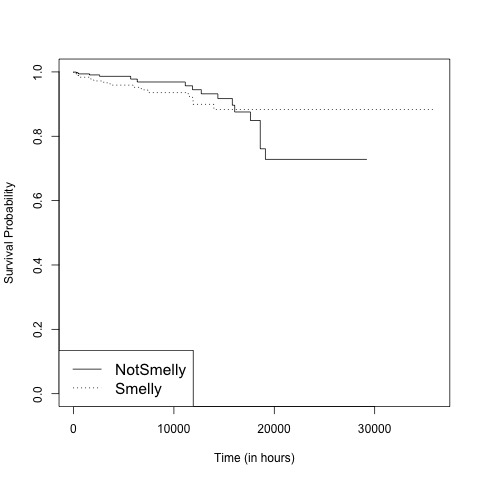
\epsfig{file = pdfs/Express_vulnerabilities_smells_file-grain_rplot.jpg, width = 4cm}}%
	}
	\subfigure[request.js]{%
		{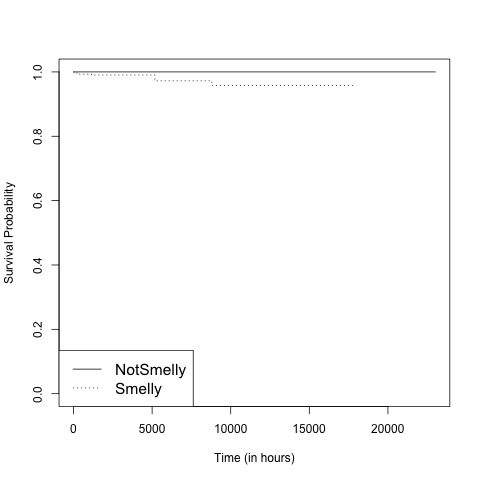
\epsfig{file = pdfs/Request_vulnerabilities_smells_file-grain_rplot.jpg, width = 4cm}}%
	}
	\subfigure[grunt.js]{%
		{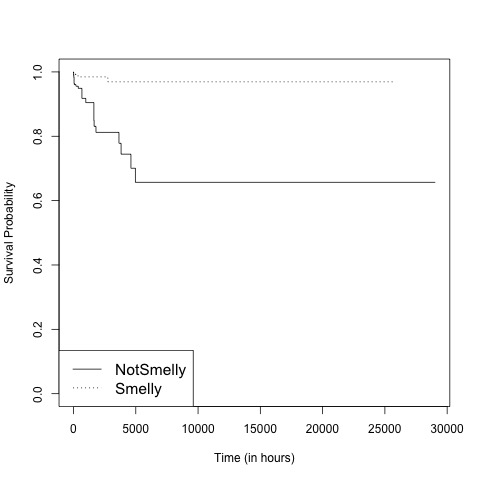
\epsfig{file = pdfs/Grunt_vulnerabilities_smells_file-grain_rplot.jpg, width = 4cm}}%
	}
	\subfigure[bower.js]{%
		{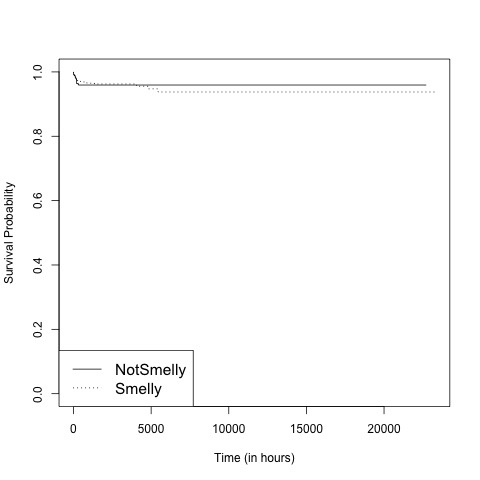
\epsfig{file = pdfs/Bower_vulnerabilities_smells_file-grain_rplot.jpg, width = 4cm}}%
	}
	\subfigure[hexo.js]{%
		{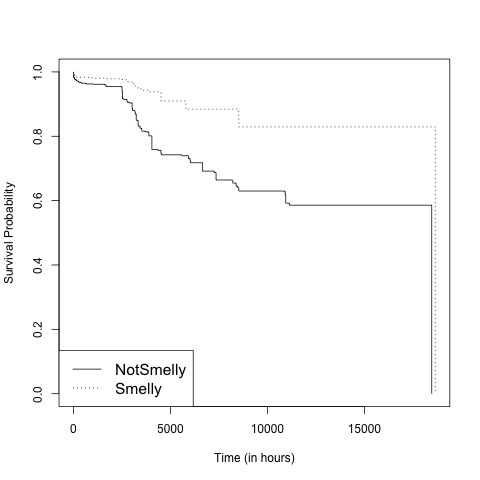
\epsfig{file = pdfs/Hexo_vulnerabilities_smells_file-grain_rplot.jpg, width = 4cm}}%
	}
	\subfigure[riot.js]{%
		{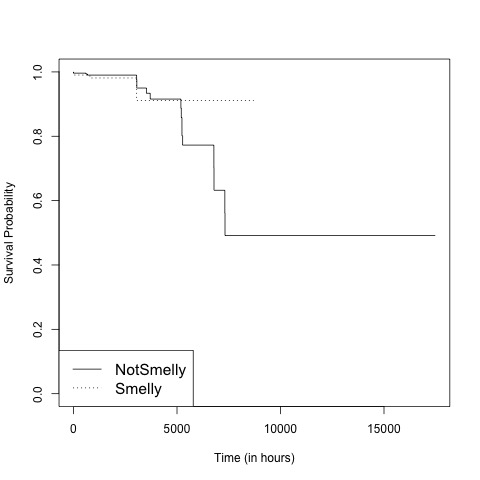
\epsfig{file = pdfs/Riot_vulnerabilities_smells_file-grain_rplot.jpg, width = 4cm}}%
	}
	\subfigure[webpack.js]{%
		{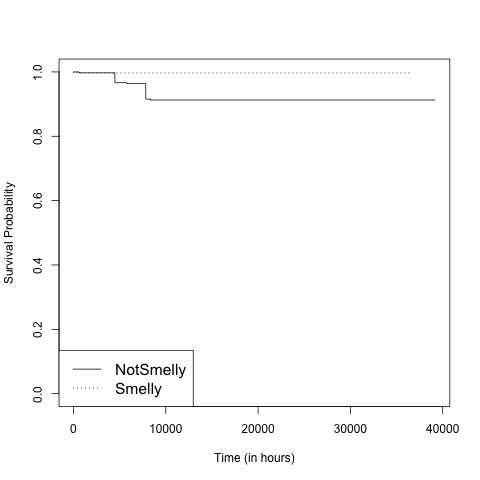
\epsfig{file = pdfs/Webpack_vulnerabilities_smells_file-grain_rplot.jpg, width = 4cm}}%
	}
	\subfigure[webtorrent.js]{%
		{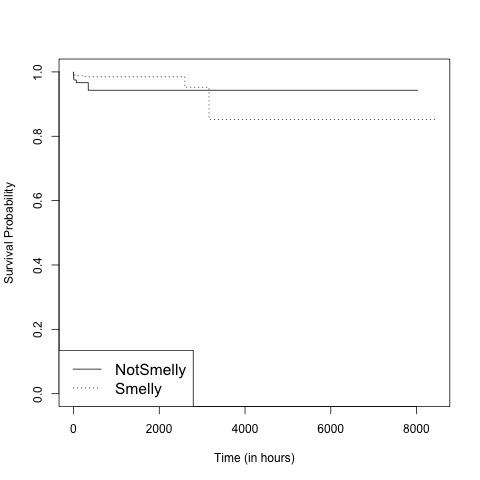
\epsfig{file = pdfs/Webtorrent_vulnerabilities_smells_file-grain_rplot.jpg, width = 4cm}}%
	}
	\caption{Survival probability trends of smelly codes vs. non-smelly codes in our fifteen JavaScript projects with the file grain approach (vulnerability study).\vspace{-10pt}}
	\label{rq3}
\end{figure*}

\begin{table*}[t]
	\centering
	\scriptsize
	\caption{Hazard ratios (vulnerability study) for each project with the line grain approach. $exp(coef)$ values means higher hazard rates.}
	\label{vulnlinegrain}
	\begin{tabular}{l|l|l|l}
		\hline
		module & $exp(coef)$ & $p$-value (Cox hazard model) & $p$-value (Proportional hazards assumption)     \\ \hline
		express  & 0.288 & 0.082e-3 & 0.113 \\ \hline
		request  & 0.189 & 0.014 & 0.441 \\ \hline
		bower	 & 0.229 & 0.031e-7 & 0.021 \\ \hline
		grunt    & 0.043 & 0.023e-7 & 0.994 \\ \hline
		hexo	 & 0.287 & 0.056e-14 & 0.902 \\ \hline
		webpack	 & 0.142 & 0.047e-3 & 0.089 \\ \hline
		webtorrent & 0.175 & 0.097e-3 & 0.217 \\ \hline
		riot	 & 0.774 & 0.445 & 0.505 \\ \hline
	\end{tabular}

\end{table*}

\begin{table*}[t]
	\centering
	\scriptsize
	\caption{Hazard ratios (vulnerability study) for each project with the line grain including dependencies approach. $exp(coef)$ values means higher hazard rates.}
	\label{vulnlinegraindep}
	\begin{tabular}{l|l|l|l}
		\hline
		module & $exp(coef)$ & $p$-value (Cox hazard model) & $p$-value (Proportional hazards assumption)     \\ \hline
		express  & 0.489 & 0.013 & 0.066 \\ \hline
		request  & 0.831 & 0.818 & 0.667 \\ \hline
		bower	 & 0.243 & 0.013e-6 & 0.009 \\ \hline
		grunt    & 0.096 & 0.03e-7 & 0.58 \\ \hline
		hexo	 & 0.322 & 0.04e-12 & 0.896 \\ \hline
		webpack	 & 0.176 & 0.09e-3 & 0.059 \\ \hline
		webtorrent & 0.31 & 0.009 & 0.109 \\ \hline
		riot	 & 0.774 & 0.445 & 0.505 \\ \hline
	\end{tabular}

\end{table*}

\textbf{Approach}. We use here our framework described in Section~\ref{extraction} {\color{blue}(Figure~\ref{process2})} to collect information about the occurrence of the 12 studied code smells in our {\color{blue}fifteen} subject systems, as well as the vulnerable codes and commits.
For each file and for each revision $r$ (\ie{} corresponding to a commit), we also compute the \textbf{Time} and \textbf{Smelly} metrics defined in \textbf{RQ1}. We also compute the \textbf{Event}, but differently to \textbf{RQ1}: for the file grain approach, this metric takes the value $1$ if the revision $r$ introduces a vulnerability $v$ for the first time through its changes and $0$ otherwise. Indeed, We only take in account the revision $r$ in which the vulnerability $v$ appears for the first time. We use the SZZ algorithm to insure that the file contained a code smell when the vulnerability was introduced for the first time. For the line grain and line grain including dependencies approaches, this metric takes the value $1$ if the revision $r$ introduces the vulnerability $v$ for the first time and if there is at least one match between the vulnerable lines and the smell lines, and $0$ otherwise. Actually, if there is no matching, we say that there is no link between the changes that inroduce the vulnerability for the first time and the code smells.

To collect information about vulnerabilities of revisions, we question a specific vulnerability database, Snyk\footnote{https://snyk.io/test}, which gives us the vulnerabilities's characteristics of each revision and of each studied systems. However, this database is not complete, which poses two problems to keep in mind during our study:
\begin{itemize}
	\item Given a studied system, some of its revisions are not identified in the database. We often meet a situation in which three successive revisions should introduce a same vulnerability, but the intermediate one indexes no vulnerability because it is not recognized by the database.
	\item Some of our studied systems (more precisely seven, which means almost half) have no vulnerability. However, we are aware that this kind of system (which means large system) are unlikely to have no vulnerability. Thereby, we will focus our analyzes on the following eight systems: \textsl{bower}, \textsl{express}, \textsl{grunt}, \textsl{hexo}, \textsl{request}, \textsl{riot}, \textsl{webpack}, and \textsl{webtorrent}.
\end{itemize}
Also, this database presents another drawback, because of its low accuracy. Indeed, when a vulnerability is found by the database, it does not specify any file of the revision in which the vulnerability has been found. Thus, we can only suppose that the vulnerability affects all the files changed by the revision, which is not accurate.

Using the smelly metric, in a similar way than \textbf{RQ1}, we divide our dataset in two groups: one group containing files with code smells (\ie{} smelly = 1) and another group containing files without any of the 12 studied code smells (\ie{} smelly = 0). For each group we create an individual Cox hazard model. In each group, the covariate of interest (\ie{} smelly) is a constant function (with value either 1 or 0), hence, there is no need for a link function to establish a linear relationship between this covariate and our event of interest, \ie{} the first appearance of a vulnerability. We use the \textsl{survfit} and \textsl{coxph} functions from R~\cite{rPackage} to analyze our Cox hazard models.

In addition to building Cox hazard models, we test the following null hypothesis: \emph{$H^{2}_{0}$: There is no difference between the probability of a first vulnerability occurrence in a file containing code smells and a file without code smells}. We use the \textsl{log-rank} test (which compares the survival distributions of two samples), to accept or refute this null hypothesis.

\textbf{Findings}. File grain results presented in Figure~\ref{rq3} show that files containing code smells don't necessarily experience vulnerability faster than files without code smells (only \textsl{request} and \textsl{bower} show that files containing smells have a trend to be more vulnerable than files without smells). Table~\ref{vulnlinegrain} (line grain results) and~\ref{vulnlinegraindep} (line grain including dependencies results) show the same accentuated observation, because none of the \textsl{exp(coef)} is greater than $1$. The $Y$-axis in Figure~\ref{rq3} represents the probability of a file \emph{surviving} a vulnerability occurrence. Hence a low value on the $Y$-axis means a low \emph{survival} rate (\ie{} a high vulnerability or high risk of vulnerability occurrence).  
For all fifteen projects, and for each approach (file grain, line grain, and line grain including dependencies), we calculated relative fault hazard rates (using Equation~\ref{eq3} from Section~\ref{survival}) between files containing code smells and files without code smells. Results show that, on average, files without code smells have hazard rates 34\% upper than files with code smells in our file grain analysis, and this pourcentage increases with the others analyzes (line grain and line grain including dependencies). Nevertheless, we need to be careful with our conclusion because of the lack of completeness and accuracy of our vulnerability database, as said previously. Hence, we can not reject $H^{2}_{0}$ because of our \textsl{exp(coef)} results, but we can not validate it because of the weaknesses of the vulnerability database we used.

\hypobox{JavaScript files with code smells are not necessarily more vulnerable than JavaScript files without code smells, and we need a better vulnerability database to confirm or refute more precisely our conclusion.}

\subsection*{(RQ4) Are JavaScript files with code smells equally vulnerable?}

\begin{table}[t]
	\centering
	\scriptsize
	\caption{Hazard ratios (vulnerability study) for each type of code smells with file grain approach. Higher $exp(coef)$ values means higher hazard rates.}
	\begin{tabular}{c|c|c|p{1.1cm}|p{1.3cm}}
		\hline
		module & covariate & $exp(coef)$ & $p$-value (Cox hazard model) & $p$-value (Proportional hazards assumption) \\ \hline
		\multirow{1}{*}{grunt} 
		& Variable Re-assign & 0.178 & 0.057e-5 & 0.169 \\ \hline
		\multirow{2}{*}{request}
		& LOC & 1.002 & 0.001 & 0.935 \\ \cline{2-5}
		& This Assign & 4.707 & 0.03 & 0.52 \\ \hline
		\multirow{2}{*}{hexo}
		& This Assign & 0.41 & 0.02 & 0.275 \\ \cline{2-5}
		& Variable Re-assign & 0.407 & 0.074e-8 & 0.668 \\ \hline
		\multirow{1}{*}{riot}
		& This Assign & 2.76 & 0.026 & 0.974 \\ \hline
		\multirow{1}{*}{webpack}
		& LOC & 1.001 & 0.009 & 0.465 \\ \hline
	\end{tabular}
	\label{smelltypes4}

\end{table}

\begin{table}[t]
	\centering
	\scriptsize
	\caption{Hazard ratios (vulnerability study) for each type of code smells with line grain approach. Higher $exp(coef)$ values means higher hazard rates.}
	\begin{tabular}{c|c|c|p{1.1cm}|p{1.3cm}}
		\hline
		module & covariate & $exp(coef)$ & $p$-value (Cox hazard model) & $p$-value (Proportional hazards assumption) \\ \hline
		\multirow{1}{*}{express}
		& Variable Re-assign & 0.342 & 0.001 & 0.08  \\ \hline
		\multirow{1}{*}{grunt} 
		& Variable Re-assign & 0.047 & 0.059e-7 & 0.996 \\ \hline
		\multirow{1}{*}{bower}
		& This Assign & 0.283 & 0.015 & 0.756 \\ \hline
		\multirow{2}{*}{request}
		& LOC & 1.002 & 0.001 & 0.935 \\ \cline{2-5}
		& Variable Re-assign & 0.228 & 0.028 & 0.426 \\ \hline
		\multirow{3}{*}{hexo}
		& This Assign & 0.291 & 0.006 & 0.377 \\ \cline{2-5}
		& Chained Methods & 0.2 & 0.023 & 0.593 \\ \cline{2-5}
		& Variable Re-assign & 0.297 & 0.014e-12 & 0.868 \\ \hline
		\multirow{2}{*}{webpack}
		& LOC & 1.001 & 0.009 & 0.465 \\ \cline{2-5}
		& Variable Re-assign & 0.146 & 0.061e-3 & 0.088 \\ \hline
		\multirow{1}{*}{webtorrent}
		& Variable Re-assign & 0.24 & 0.002 & 0.183 \\ \hline
	\end{tabular}
	\label{smelltypes5}

\end{table}

\begin{table}[t]
	\centering
	\scriptsize
	\caption{Hazard ratios (vulnerability study) for each type of code smells with line grain including dependencies approach. Higher $exp(coef)$ values means higher hazard rates.}
	\begin{tabular}{c|c|c|p{1.1cm}|p{1.3cm}}
		\hline
		module & covariate & $exp(coef)$ & $p$-value (Cox hazard model) & $p$-value (Proportional hazards assumption) \\ \hline
		\multirow{1}{*}{grunt} 
		& Variable Re-assign & 0.088 & 0.057e-7 & 0.581 \\ \hline
		\multirow{1}{*}{bower}
		& This Assign & 0.283 & 0.015 & 0.756 \\ \hline
		\multirow{1}{*}{request}
		& LOC & 1.002 & 0.001 & 0.935 \\ \hline
		\multirow{2}{*}{hexo}
		& This Assign & 0.291 & 0.006 & 0.377 \\ \cline{2-5}
		& Variable Re-assign & 0.327 & 0.035e-11 & 0.972 \\ \hline
		\multirow{2}{*}{webpack}
		& LOC & 1.001 & 0.009 & 0.465 \\ \cline{2-5}
		& Variable Re-assign & 0.181 & 0.012e-2 & 0.058 \\ \hline
	\end{tabular}
	\label{smelltypes6}

\end{table}

\textbf{Approach}. Similar to \textbf{RQ3}, we use our framework from Section~\ref{extraction} (Figure~\ref{process2}) to collect information about the occurrence of the 12 studied code smells, as well as the vulnerable codes and commits, in our fifteen studied systems. For each file and for each revision $r$ (\ie{} corresponding to a commit), we also compute the \textbf{Time} and \textbf{Event} metrics defined in \textbf{RQ3}. For each type of code smell $i$ we define the metric \textbf{Smelly$_{i}$:} which takes the value $1$ if the revision $r$ of the file contains the code smell $i$ and $0$ if it doesn't contain any of the 12 studied code smells. Also, for the line grain and the line grain including dependencies approaches, we define the metric \textbf{Event$_{i}$:} which takes the value $1$ if the revision $r$ introduces a vulnerability $v$ for the first time through its changes and if the code smell $i$ is in the intersection between the vulnerability lines and the smell lines, and $0$ otherwise. When computing the \textbf{Event} and \textbf{Event$_{i}$} metrics, we used the SZZ algorithm to ensure that the file contained the code smell $i$ when the vulnerability was introduced.
Because size and code churn could be related to vulnerability, we add the following metrics to our models, to control for the effect of these covariates : (i) LOC: the number of lines of code in the file at revision $r$; (ii) Code Churn: the sum of added, removed and modified lines in the file prior to revision $r$.

We perform a stratification considering the covariates mentioned above, in order to monitor their effect on our event of interest, \ie{} a vulnerability occurrence. Next, we create a Cox hazard model for each of our fifteen studied systems.
We then generated summaries of all our Cox hazard models and removed insignificant covariates, \ie{} those with $p$-values greater than $0.05$. Finally, for each system, we performed a non-proportional test to verify if the proportional hazards assumption holds. 

\textbf{Findings}. Tables~\ref{smelltypes4},~\ref{smelltypes5} and~\ref{smelltypes6} summarize the vulnerability hazard ratios for the 12 studied code smells for respectively the file grain, line grain, and line grain including dependencies approach. The value in the column \textsl{exp(coef)} shows the amount of increase in vulnerability hazard rate that one should expect for each unit increase in the value of the corresponding covariate.
The last column of Tables~\ref{smelltypes4},~\ref{smelltypes5} and~\ref{smelltypes6} show that the $p$-values obtained for the non-proportionality tests are above $0.05$ for all the fifteen systems; meaning that the proportional hazards assumption is satisfied for all the fifteen studied systems. Actually, we removed from the tables the insignificant covariates, which means those with non-proportionality test $p$-values less than $0.05$.

Overall, the vulnerability hazard ratios of the studied code smells vary across the systems and accross the approaches (file grain, line grain and line grain including dependencies), and almost all of them have an \textsl{exp(coef)} less than $1$. It confirms our last conclusion in \textbf{RQ3}, that is to say that JavaScript files with code smells are not more vulnerable than those without code smells (and we still have to mitigate this conclusion because of our vulnerability database). As said in \textbf{RQ3}, we collected information only on eight systems (out of fifteen) because of the lack of completeness of the vulnerability database. Plus, because of our $p$-values restriction, only a few covariates are reported in our tables, and some of the eight studied systems don't appear. However, it is interesting to notice that with the file grain approach, \textsl{This Assign} has the highest vulnerability hazard ratio in three out of eight systems (37.5\%), and is the only covariate with a hazard ratio greater than $1$ in two systems (\textsl{request} and \textsl{riot}); \textsl{Variable Re-assign} has one of the highest hazard rate in two out of eight systems (25\%); \textsl{This Assign} and \textsl{Variable Re-assign} are the only smell covariates reported. With our line grain approach, \textsl{Variable Re-assign} has still one of the highest hazard ratio in most systems, that is to say in six out of eight systems (75\%); \textsl{This Assign} has one of the highest hazard rate in two out of eight systems (25\%); \textsl{Chained Methods} is the most hazard code smell in only one out of eight systems (12.5\%); the other smells don't appear in any of the studied systems because of the $p$-values limitations. With the line grain including dependencies approach, \textsl{Variable Re-assign} is still one of the most hazard code smell in most systems, in three out of fifteen systems (37.5\%); \textsl{This Assign}  has one of the highest hazard rate in two out of eight systems (25\%); and only \textsl{Variable Re-assign} and \textsl{This Assign} are reported. Furthemore, the most vulnerability hazard types of code smell seem not to vary accross the approaches, and this observation particularly affects \textsl{Variable Re-assign} and \textsl{This Assign} code smells.

In our three approaches, the covariate LOC is significantly related to fault occurrence in two systems (\textsl{request} and \textsl{webpack}) with a very low hazard rate, meaning that JavaScript developers cannot simply control for size if they want to track vulnerable files effectively. Since \textsl{Variable Re-assign} and \textsl{This Assign} have the highest hazard ratios in respectively 46\% and 29\% of the cases (which means eight studied systems and three approches, that is to say $24$ cases), we can recommend that developers prioritize files containing these two types of code smells in order to make their system less vulnerable. \textsl{Variable Re-assign} seems, as in \textbf{RQ2}, an unavoidable type smell that developers have to strongly consider when they maintain, test, and fix their system for reducing fault-proneness and potentially vulnerability.

\hypobox{JavaScript files containing different types of code smells are not equally vulnerable. Developers should consider refactoring files containing \textsl{Variable Re-assign} code smell or \textsl{This Assign} code smell in priority since they seem to increase the risk of vulnerability in the system. Finally, \textsl{Variable Re-assign} code smell is essential to consider for reducing the risk of vulnerability and fault in the system.}

\subsection*{(RQ5) How do the smells survive over time?}

\begin{table*}[!htbp]
	\centering

	\caption{Descriptive statistics on survival over time of the largest smells of studied systems.}
	\begin{tabular}{c|c|c|c|c|c|c}
		\hline
		System & Smell & Not Survived & Survived & Number created at file birth & Median days or survival & Average days of survival \\ \hline
		\multirow{5}{*}{express}
		& Variable Re-assign & 6743 & 425 & 5783 (80.7\%) & 74 & 209 \\ \cline{2-7}
		& Nested Callbacks & 314 & 728 & 417 (40\%) & 1101 & 1152 \\ \cline{2-7}
		& Complex Code & 374 & 5 & 353 (93.1\%) & 74 & 122 \\ \cline{2-7}
		& Long Methods & 283 & 9 & 260 (89\%) & 74 & 143 \\ \cline{2-7}
		& SUM & 8430 & 1238 & 7348 (76\%) & & \\ \hline
		\multirow{5}{*}{grunt} 
		& Variable Re-assign & 2210 & 317 & 1636 (64.7\%) & 248 & 411 \\ \cline{2-7}
		& Lengthy Lines & 243 & 108 & 172 (49\%) & 248 & 681 \\ \cline{2-7}
		& Complex Code & 91 & 5 & 83 (85.4\%) & 248 & 292 \\ \cline{2-7}
		& Long Methods & 55 & 5 & 41 (68.3\%) & 248 & 334 \\ \cline{2-7}
		& SUM & 2732 & 448 & 2017 (63.4\%) & & \\ \hline
		\multirow{5}{*}{bower}
		& Variable Re-assign & 1427 & 1801 & 1235 (38.3\%) & 797 & 777 \\ \cline{2-7}
		& Chained Methods & 82 & 96 & 35 (19.7\%) & 1231 & 819 \\ \cline{2-7}
		& Lengthy Lines & 32 & 50 & 28 (34.1\%) & 644 & 719 \\ \cline{2-7}
		& Nested Callbacks & 38 & 32 & 27 (38.6\%) & 163 & 656 \\ \cline{2-7}
		& SUM & 1647 & 2087 & 1368 (36.6\%) & & \\ \hline
		\multirow{5}{*}{less}
		& Variable Re-assign & 36979 & 3779 & 37303 (91.5\%) & 56 & 281 \\ \cline{2-7}
		& Assign. in Cond. State. & 1349 & 4 & 1261 (93.2\%) & 405 & 477 \\ \cline{2-7}
		& Lengthy Lines & 547 & 26 & 509 (88.8\%) & 36 & 139 \\ \cline{2-7}
		& This Assign & 392 & 33 & 387 (91.1\%) & 129 & 314 \\ \cline{2-7}
		& SUM & 40241 & 3927 & 40391 (91.4\%) & & \\ \hline
		\multirow{5}{*}{request}
		& Variable Re-assign & 1362 & 667 & 1140 (56.2\%) & 365 & 534 \\ \cline{2-7}
		& This Assign & 28 & 50 & 34 (43.6\%) & 874 & 743 \\ \cline{2-7}
		& Chained Methods & 32 & 22 & 38 (70.4\%) & 256 & 557 \\ \cline{2-7}
		& Nested Callbacks & 1 & 28 & 1 (3.4\%) & 774 & 592 \\ \cline{2-7}
		& SUM & 1455 & 777 & 1232 (55.2\%) & & \\ \hline
		\multirow{5}{*}{jquery}
		& Variable Re-assign & 13076 & 5156 & 12122 (66.5\%) & 528 & 694 \\ \cline{2-7}
		& Complex Switch Case & 146 & 15 & 130 (80.7\%) & 179 & 435 \\ \cline{2-7}
		& This Assign & 118 & 37 & 120 (77.4\%) & 539 & 716 \\ \cline{2-7}
		& Chained Methods & 59 & 58 & 35 (29.9\%) & 657 & 785 \\ \cline{2-7}
		& SUM & 13743 & 5356 & 12675 (66.4\%) & & \\ \hline
		\multirow{5}{*}{hexo}
		& Variable Re-assign & 19023 & 823 & 17626 (88.8\%) & 2 & 86 \\ \cline{2-7}
		& Lengthy Lines & 768 & 12 & 675 (86.5\%) & 10 & 138 \\ \cline{2-7}
		& Long Parameter List & 755 & 3 & 728 (96\%) & 2 & 20 \\ \cline{2-7}
		& Complex Code & 599 & 19 & 576 (93.2\%) & 2 & 51 \\ \cline{2-7}
		& SUM & 22522 & 980 & 20584 (87.6\%) & & \\ \hline
		\multirow{5}{*}{leaflet}
		& Variable Re-assign & 5856 & 498 & 2241 (35.3\%) & 789.5 & 734 \\ \cline{2-7}
		& Lengthy Lines & 733 & 270 & 358 (35.7\%) & 203 & 354 \\ \cline{2-7}
		& Nested Callbacks & 123 & 489 & 114 (18.6\%) & 986 & 1029 \\ \cline{2-7}
		& Long Methods & 77 & 5 & 32 (39\%) & 911 & 752 \\ \cline{2-7}
		& SUM & 6997 & 1278 & 2855 (34.5\%) & & \\ \hline
		\multirow{5}{*}{ramda}
		& Variable Re-assign & 4720 & 1078 & 4656 (80.3\%) & 375 & 391 \\ \cline{2-7}
		& Chained Methods & 365 & 101 & 344 (73.8\%) & 241 & 372 \\ \cline{2-7}
		& Long Parameter List & 176 & 90 & 208 (78.2\%) & 206 & 396 \\ \cline{2-7}
		& Complex Code & 194 & 28 & 200 (90.1\%) & 375 & 364 \\ \cline{2-7}
		& SUM & 5668 & 1340 & 5599 (79.9\%) & & \\ \hline
		\multirow{5}{*}{chart}
		& Variable Re-assign & 5297 & 5696 & 4538 (41.3\%) & 406 & 365 \\ \cline{2-7}
		& This Assign & 199 & 388 & 86 (14.7\%) & 406 & 339 \\ \cline{2-7}
		& Lengthy Lines & 119 & 14 & 34 (25.6\%) & 12 & 154 \\ \cline{2-7}
		& Complex Switch Case & 53 & 30 & 31 (37.3\%) & 169 & 258 \\ \cline{2-7}
		& SUM & 5740 & 6207 & 4746 (39.7\%) & & \\ \hline
		\multirow{5}{*}{riot}
		& Variable Re-assign & 8331 & 2625 & 7866 (71.9\%) & 52 & 188 \\ \cline{2-7}
		& Lengthy Lines & 193 & 33 & 206 (91.2\%) & 7 & 150 \\ \cline{2-7}
		& This Assign & 63 & 92 & 61 (39.4\%) & 43 & 110 \\ \cline{2-7}
		& Assign. in Cond. State. & 107 & 47 & 80 (51.9\%) & 100.5 & 196 \\ \cline{2-7}
		& SUM & 9119 & 2937 & 8637 (71.6\%) & & \\ \hline
		\multirow{5}{*}{vue}
		& Variable Re-assign & 4199 & 5833 & 6587 (65.7\%) & 139 & 175 \\ \cline{2-7}
		& Lengthy Lines & 2947 & 4208 & 3518 (49.2\%) & 125 & 143 \\ \cline{2-7}
		& Complex Code & 414 & 675 & 679 (62.4\%) & 139 & 171 \\ \cline{2-7}
		& Long Methods & 259 & 417 & 421 (62.3\%) & 139 & 171 \\ \cline{2-7}
		& SUM & 8612 & 11712 & 12129 (59.7\%) & & \\ \hline
		\multirow{5}{*}{moment}
		& Variable Re-assign & 5642 & 11063 & 6154 (36.8\%) & 450 & 486 \\ \cline{2-7}
		& Nested Callbacks & 19 & 335 & 12 (3.4\%) & 492 & 464 \\ \cline{2-7}
		& Complex Switch Case & 117 & 69 & 114 (61.3\%) & 299 & 634 \\ \cline{2-7}
		& Chained Methods & 113 & 42 & 74 (47.7\%) & 243 & 389 \\ \cline{2-7}
		& SUM & 6135 & 11590 & 6561 (37\%) & & \\ \hline
		\multirow{5}{*}{webpack}
		& Variable Re-assign & 4643 & 627 & 3192 (60.6\%) & 352 & 593 \\ \cline{2-7}
		& Nested Callbacks & 379 & 54 & 276 (63.7\%) & 104 & 359 \\ \cline{2-7}
		& Chained Methods & 371 & 16 & 174 (45\%) & 492 & 589 \\ \cline{2-7}
		& Lengthy Lines & 182 & 38 & 86 (39.1\%) & 236 & 518 \\ \cline{2-7}
		& SUM & 5970 & 813 & 3987 (58.8\%) & & \\ \hline
		\multirow{5}{*}{webtorrent}
		& Variable Re-assign & 709 & 424 & 471 (41.6\%) & 335 & 370 \\ \cline{2-7}
		& This Assign & 108 & 53 & 88 (54.7\%) & 335 & 427 \\ \cline{2-7}
		& Nested Callbacks & 28 & 55 & 23 (27.7\%) & 453 & 406 \\ \cline{2-7}
		& Chained Methods & 12 & 2 & 9 (64.3\%) & 19.5 & 122 \\ \cline{2-7}
		& SUM & 869 & 535 & 591 (42.1\%) & & \\ \hline
	\end{tabular}
	\label{survivalsmells}
\end{table*}

\begin{figure*}[!htbp]
	\centering%
	\subfigure[Variable Re-Assign]{%
		{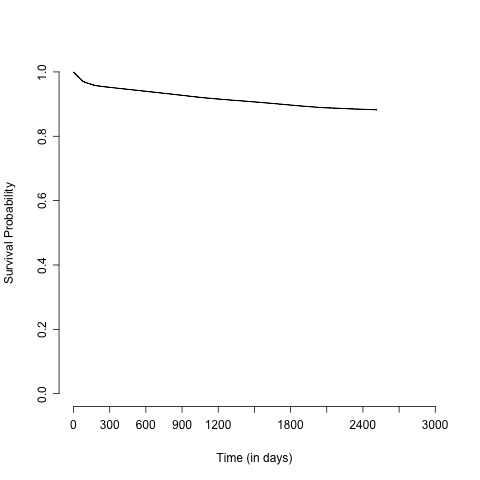
\epsfig{file = pdfs/Express_no-reassign_rplot.jpg, width = 4cm}}%
	}
	\subfigure[Nested Callbacks]{%
		{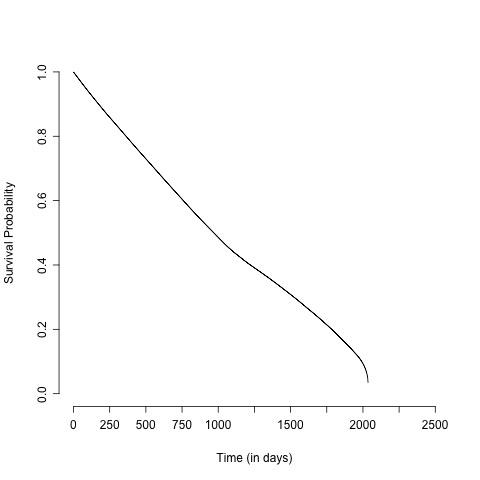
\epsfig{file = pdfs/Express_max-nested-callbacks_rplot.jpg, width = 4cm}}%
	}
	\subfigure[Complex Code]{%
		{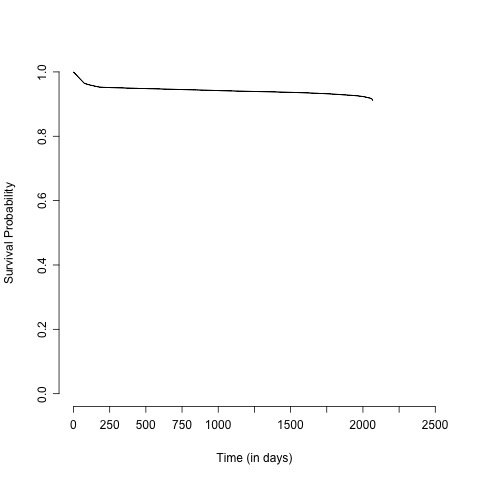
\epsfig{file = pdfs/Express_complexity_rplot.jpg, width = 4cm}}%
	}
	\subfigure[Long Methods]{%
		{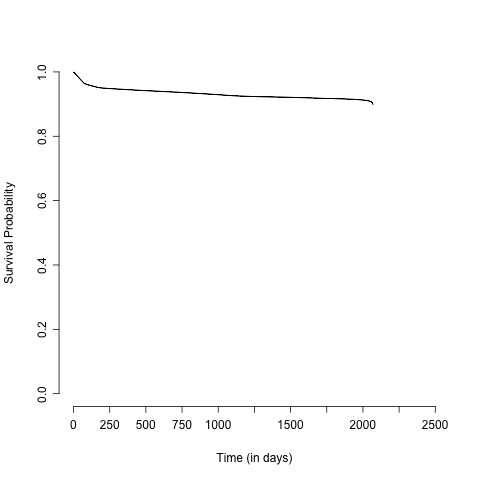
\epsfig{file = pdfs/Express_max-statements_rplot.jpg, width = 4cm}}%
	}
	\caption{Survival analyzes of the largest smells of express.js.\vspace{-10pt}}
	\label{survivalplots1}
\end{figure*}

\begin{figure*}[!htbp]
	\centering%
	\subfigure[Variable Re-Assign]{%
		{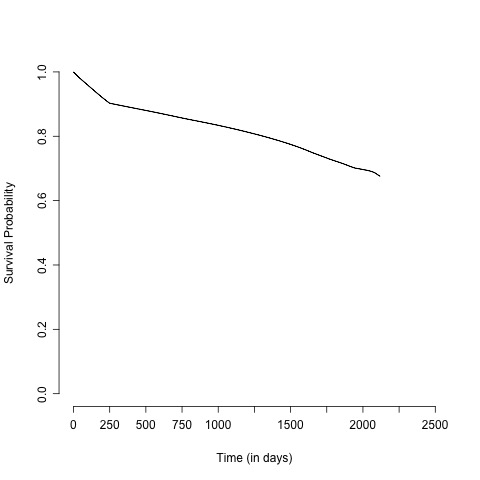
\epsfig{file = pdfs/Grunt_no-reassign_rplot.jpg, width = 4cm}}%
	}
	\subfigure[Lengthy Lines]{%
		{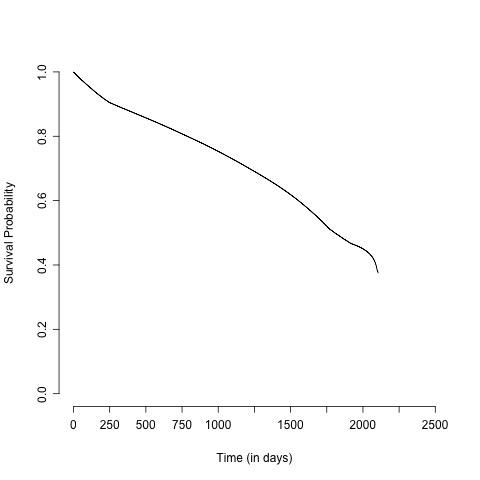
\epsfig{file = pdfs/Grunt_max-len_rplot.jpg, width = 4cm}}%
	}
	\subfigure[Complex Code]{%
		{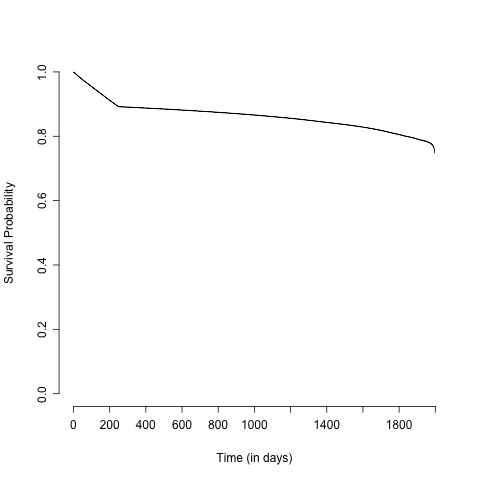
\epsfig{file = pdfs/Grunt_complexity_rplot.jpg, width = 4cm}}%
	}
	\subfigure[Long Methods]{%
		{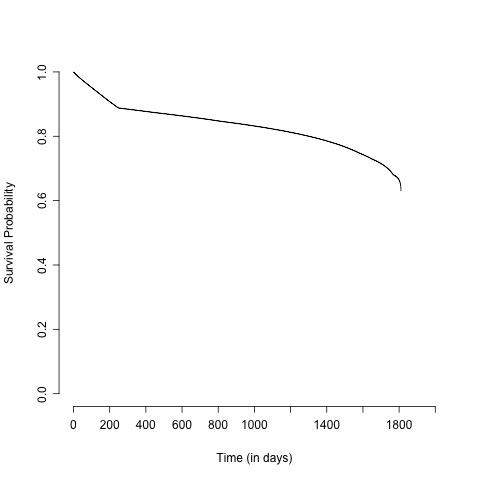
\epsfig{file = pdfs/Grunt_max-statements_rplot.jpg, width = 4cm}}%
	}
	\caption{Survival analyzes of the largest smells of grunt.js.\vspace{-10pt}}
	\label{survivalplots2}
\end{figure*}

\begin{figure*}[!htbp]
	\centering%
	\subfigure[Variable Re-Assign]{%
		{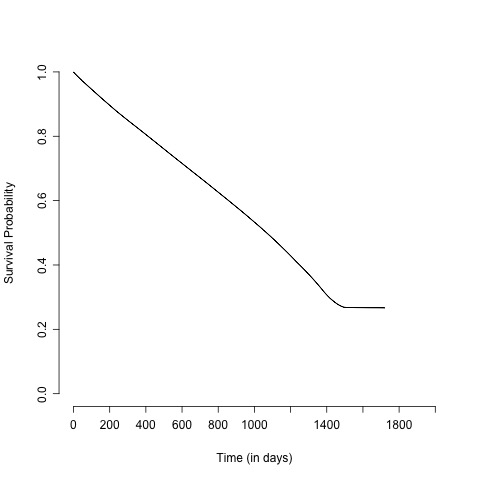
\epsfig{file = pdfs/Bower_no-reassign_rplot.jpg, width = 4cm}}%
	}
	\subfigure[Chained Methods]{%
		{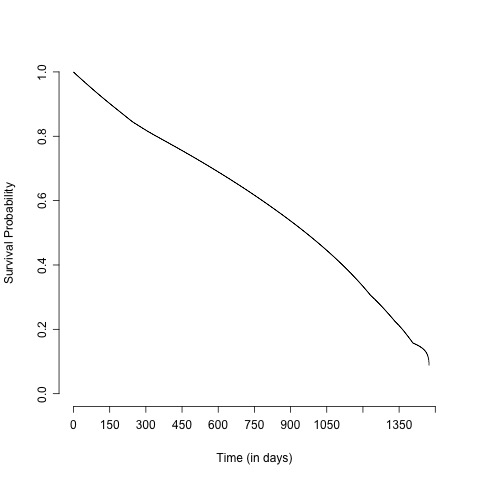
\epsfig{file = pdfs/Bower_complex-chaining_rplot.jpg, width = 4cm}}%
	}
	\subfigure[Lengthy Lines]{%
		{\epsfig{file = pdfs/Bower_max-len_rplot.jpg, width = 4cm}}%
	}
	\subfigure[Nested Callbacks]{%
		{\epsfig{file = pdfs/Bower_max-nested-callbacks_rplot.jpg, width = 4cm}}%
	}
	\caption{Survival analyzes of the largest smells of bower.js.\vspace{-10pt}}
	\label{survivalplots3}
\end{figure*}

\begin{figure*}[!htbp]
	\centering%
	\subfigure[Variable Re-Assign]{%
		{\epsfig{file = pdfs/Less_no-reassign_rplot.jpg, width = 4cm}}%
	}
	\subfigure[Nested Callbacks]{%
		{\epsfig{file = pdfs/Less_max-nested-callbacks_rplot.jpg, width = 4cm}}%
	}
	\subfigure[Complex Code]{%
		{\epsfig{file = pdfs/Less_complexity_rplot.jpg, width = 4cm}}%
	}
	\subfigure[Long Methods]{%
		{\epsfig{file = pdfs/Less_max-statements_rplot.jpg, width = 4cm}}%
	}
	\caption{Survival analyzes of the largest smells of less.js.\vspace{-10pt}}
	\label{survivalplots4}
\end{figure*}

\begin{figure*}[!htbp]
	\centering%
	\subfigure[Variable Re-Assign]{%
		{\epsfig{file = pdfs/Request_no-reassign_rplot.jpg, width = 4cm}}%
	}
	\subfigure[This Assign]{%
		{\epsfig{file = pdfs/Request_this-assign_rplot.jpg, width = 4cm}}%
	}
	\subfigure[Chained Methods]{%
		{\epsfig{file = pdfs/Request_complex-chaining_rplot.jpg, width = 4cm}}%
	}
	\subfigure[Nested Callbacks]{%
		{\epsfig{file = pdfs/Request_max-nested-callbacks_rplot.jpg, width = 4cm}}%
	}
	\caption{Survival analyzes of the largest smells of request.js.\vspace{-10pt}}
	\label{survivalplots5}
\end{figure*}

\begin{figure*}[!htbp]
	\centering%
	\subfigure[Variable Re-Assign]{%
		{\epsfig{file = pdfs/Jquery_no-reassign_rplot.jpg, width = 4cm}}%
	}
	\subfigure[Complex Switch Case]{%
		{\epsfig{file = pdfs/Jquery_complex-switch-case_rplot.jpg, width = 4cm}}%
	}
	\subfigure[This Assign]{%
		{\epsfig{file = pdfs/Jquery_this-assign_rplot.jpg, width = 4cm}}%
	}
	\subfigure[Chained Methods]{%
		{\epsfig{file = pdfs/Jquery_complex-chaining_rplot.jpg, width = 4cm}}%
	}
	\caption{Survival analyzes of the largest smells of jquery.js.\vspace{-10pt}}
	\label{survivalplots6}
\end{figure*}

\begin{figure*}[!htbp]
	\centering%
	\subfigure[Variable Re-Assign]{%
		{\epsfig{file = pdfs/Hexo_no-reassign_rplot.jpg, width = 4cm}}%
	}
	\subfigure[Lengthy Lines]{%
		{\epsfig{file = pdfs/Hexo_max-len_rplot.jpg, width = 4cm}}%
	}
	\subfigure[Long Parameter List]{%
		{\epsfig{file = pdfs/Hexo_max-params_rplot.jpg, width = 4cm}}%
	}
	\subfigure[Complex Code]{%
		{\epsfig{file = pdfs/Hexo_complexity_rplot.jpg, width = 4cm}}%
	}
	\caption{Survival analyzes of the largest smells of hexo.js.\vspace{-10pt}}
	\label{survivalplots7}
\end{figure*}

\begin{figure*}[!htbp]
	\centering%
	\subfigure[Variable Re-Assign]{%
		{\epsfig{file = pdfs/Leaflet_no-reassign_rplot.jpg, width = 4cm}}%
	}
	\subfigure[Lengthy Lines]{%
		{\epsfig{file = pdfs/Leaflet_max-len_rplot.jpg, width = 4cm}}%
	}
	\subfigure[Nested Callbacks]{%
		{\epsfig{file = pdfs/Leaflet_max-nested-callbacks_rplot.jpg, width = 4cm}}%
	}
	\subfigure[Long Methods]{%
		{\epsfig{file = pdfs/Leaflet_max-statements_rplot.jpg, width = 4cm}}%
	}
	\caption{Survival analyzes of the largest smells of leaflet.js.\vspace{-10pt}}
	\label{survivalplots8}
\end{figure*}

\begin{figure*}[!htbp]
	\centering%
	\subfigure[Variable Re-Assign]{%
		{\epsfig{file = pdfs/Ramda_no-reassign_rplot.jpg, width = 4cm}}%
	}
	\subfigure[Chained Methods]{%
		{\epsfig{file = pdfs/Ramda_complex-chaining_rplot.jpg, width = 4cm}}%
	}
	\subfigure[Long Parameter List]{%
		{\epsfig{file = pdfs/Ramda_max-params_rplot.jpg, width = 4cm}}%
	}
	\subfigure[Complex Code]{%
		{\epsfig{file = pdfs/Ramda_complexity_rplot.jpg, width = 4cm}}%
	}
	\caption{Survival analyzes of the largest smells of ramda.js.\vspace{-10pt}}
	\label{survivalplots9}
\end{figure*}

\begin{figure*}[!htbp]
	\centering%
	\subfigure[Variable Re-Assign]{%
		{\epsfig{file = pdfs/Chart_no-reassign_rplot.jpg, width = 4cm}}%
	}
	\subfigure[This Assign]{%
		{\epsfig{file = pdfs/Chart_this-assign_rplot.jpg, width = 4cm}}%
	}
	\subfigure[Lengthy Lines]{%
		{\epsfig{file = pdfs/Chart_max-len_rplot.jpg, width = 4cm}}%
	}
	\subfigure[Complex Switch Case]{%
		{\epsfig{file = pdfs/Chart_complex-switch-case_rplot.jpg, width = 4cm}}%
	}
	\caption{Survival analyzes of the largest smells of chart.js.\vspace{-10pt}}
	\label{survivalplots10}
\end{figure*}

\begin{figure*}[!htbp]
	\centering%
	\subfigure[Variable Re-Assign]{%
		{\epsfig{file = pdfs/Riot_no-reassign_rplot.jpg, width = 4cm}}%
	}
	\subfigure[Lengthy Lines]{%
		{\epsfig{file = pdfs/Riot_max-len_rplot.jpg, width = 4cm}}%
	}
	\subfigure[This Assign]{%
		{\epsfig{file = pdfs/Riot_this-assign_rplot.jpg, width = 4cm}}%
	}
	\subfigure[Assignment in Conditional Statement]{%
		{\epsfig{file = pdfs/Riot_cond-assign_rplot.jpg, width = 4cm}}%
	}
	\caption{Survival analyzes of the largest smells of riot.js.\vspace{-10pt}}
	\label{survivalplots11}
\end{figure*}

\begin{figure*}[!htbp]
	\centering%
	\subfigure[Variable Re-Assign]{%
		{\epsfig{file = pdfs/Vue_no-reassign_rplot.jpg, width = 4cm}}%
	}
	\subfigure[Lengthy Lines]{%
		{\epsfig{file = pdfs/Vue_max-len_rplot.jpg, width = 4cm}}%
	}
	\subfigure[Complex Code]{%
		{\epsfig{file = pdfs/Vue_complexity_rplot.jpg, width = 4cm}}%
	}
	\subfigure[Long Methods]{%
		{\epsfig{file = pdfs/Vue_max-statements_rplot.jpg, width = 4cm}}%
	}
	\caption{Survival analyzes of the largest smells of vue.js.\vspace{-10pt}}
	\label{survivalplots12}
\end{figure*}

\begin{figure*}[!htbp]
	\centering%
	\subfigure[Variable Re-Assign]{%
		{\epsfig{file = pdfs/Moment_no-reassign_rplot.jpg, width = 4cm}}%
	}
	\subfigure[Nested Callbacks]{%
		{\epsfig{file = pdfs/Moment_max-nested-callbacks_rplot.jpg, width = 4cm}}%
	}
	\subfigure[Complex Switch Case]{%
		{\epsfig{file = pdfs/Moment_complex-switch-case_rplot.jpg, width = 4cm}}%
	}
	\subfigure[Chained Methods]{%
		{\epsfig{file = pdfs/Moment_complex-chaining_rplot.jpg, width = 4cm}}%
	}
	\caption{Survival analyzes of the largest smells of moment.js.\vspace{-10pt}}
	\label{survivalplots13}
\end{figure*}

\begin{figure*}[!htbp]
	\centering%
	\subfigure[Variable Re-Assign]{%
		{\epsfig{file = pdfs/Webpack_no-reassign_rplot.jpg, width = 4cm}}%
	}
	\subfigure[Nested Callbacks]{%
		{\epsfig{file = pdfs/Webpack_max-nested-callbacks_rplot.jpg, width = 4cm}}%
	}
	\subfigure[Chained Methods]{%
		{\epsfig{file = pdfs/Webpack_complex-chaining_rplot.jpg, width = 4cm}}%
	}
	\subfigure[Lengthy Lines]{%
		{\epsfig{file = pdfs/Webpack_max-len_rplot.jpg, width = 4cm}}%
	}
	\caption{Survival analyzes of the largest smells of webpack.js.\vspace{-10pt}}
	\label{survivalplots14}
\end{figure*}

\begin{figure*}[!htbp]
	\centering%
	\subfigure[Variable Re-Assign]{%
		{\epsfig{file = pdfs/Webtorrent_no-reassign_rplot.jpg, width = 4cm}}%
	}
	\subfigure[This Assign]{%
		{\epsfig{file = pdfs/Webtorrent_this-assign_rplot.jpg, width = 4cm}}%
	}
	\subfigure[Nested Callbacks]{%
		{\epsfig{file = pdfs/Webtorrent_max-nested-callbacks_rplot.jpg, width = 4cm}}%
	}
	\subfigure[Chained Methods]{%
		{\epsfig{file = pdfs/Webtorrent_complex-chaining_rplot.jpg, width = 4cm}}%
	}
	\caption{Survival analyzes of the largest smells of webtorrent.js.\vspace{-10pt}}
	\label{survivalplots15}
\end{figure*}

\textbf{Approach}. We use now the framework described in Section~\ref{extraction}, Figure~\ref{process3}, to collect information about the appearance of the 12 studied code smells in our fifteen subject systems, as well as their line localization, their content and their genealogy (which means their evolution over time from their creation to either their destruction, or the last revision of the studied system).
For each studied system and for each smell type, we compute the following metrics:
\begin{itemize}
	\item The number of created smells.
	\item The number of killed smells (over the system lifetime).
	\item The number of survived smells, which means the number of smell that presently appear in the system.
	\item The number of smells created at the file birthdate.
	\item The median days of survival of the smells.
	\item The average days of survival of the smells.
\end{itemize}
For each smell created (which means never encountered before), we also compute the \textbf{Time} and \textbf{Event} metrics thus defined: 
\begin{itemize}
	\item \textbf{Time:} the time in days since the smell creation.
	\item \textbf{Event:} this metric takes the value $1$ if the studied smell is present at this time (which means not killed), and $0$ otherwise.
\end{itemize}
In this way, if a particular smell $s$ is killed $x$ days after its introduction, we will have the corresponding event metric equal to $1$ from $0$ to $x-1$, and equal to $0$ at the time $x$ and after. When we report those information for a studied system, the maximum time that we take in account, for a particular smell type, corresponds to the maximum lifetime of the smells of this type. Thereby, for each smell type of the system and for each time, we will know the proportion of smells alive relatively to the number of smells created. This will particularly help us in the Cox survival model design.

Then, for each of the twelve studied smells, and for each of the fifteen studied systems, we create an individual Cox survival model using the \textbf{Time} and \textbf{Event} metrics previously defined. We use the \textsl{survfit} and \textsl{coxph} functions from R~\cite{rPackage} to analyze our Cox survival models.

\textbf{Findings}. Our results are presented in the Table~\ref{survivalsmells} for a density analysis, and in the Figures~\ref{survivalplots1} to~\ref{survivalplots15} for a survival analysis. 
For the Table~\ref{survivalsmells}, for each system and each smell, the third column corresponds to the number of killed smells, and the fourth to the number of survived smells. The sum of both columns gives us the number of created smells. The fifth column reports, in pourcentage, the proportion of smells created at the files birthdate, relatively to the number of created smells. In order to not overload the presentation of our results, we only report the descriptive statistics for the four most relevant smells, which means those for wich the number created is the most considerable. Finally, the Table reports, for each studied system, general statistics (\textsl{SUM} lines), computed by summing the statistics of the twelve studied smells.
For the Figures~\ref{survivalplots1} to~\ref{survivalplots15}, we plot the survival analysis for each studied systems, and for each smells reported in the Table~\ref{survivalsmells}, still in order to not overload the presentation of our results. The $Y$-axis corresponds to the chance of surviving of a given smell type, $x$ days after its introduction into the codebase.
The results presented in Table~\ref{survivalsmells} show that smells are not often introduced during files evolution and changes, but rather at the creation of files. Indeed, when we look at the \textsl{SUM} lines, from 34.5\% (for \textsl{leaflet}) to 91.4\% (for \textsl{less}) of the smells are introduced at the file birthdate, meaning that developers should be aware to their code when they create a JavaScript file, because it is precisely at this moment that most of the smells are introduced into the system. We also notice that, for the major part of the studied systems (eight out of fifteen), more than 20\% of the smells created still survive presently; and for thirteen systems, over than 10\% of the smells created are now present in those systems. It reveals that a significant part of the smells are never removed from the system once they are introduced in the code. Plus, after analyzing the commits of the studied systems, it is interesting to notice that most of time, the killed smells are removing at the same time than the file containing them (and not because of a file fix). The Table gives us also an overview of the smells lifetime, and we observe that for most of the systems (nine out of fifteen), the median and average days of survival of the most significant smell types are greater than $100$ days; and for fourteen systems out of fifteen (except \textsl{hexo}), at least one of the most sizable smell types has an average and median lifetime greater than $100$ days. This observation highlights that in general, smells tend to survive a very long time inside the system once they are introduced. Finally, Table~\ref{survivalsmells} presents an interesting result, which is that the smell \textsl{Variable Re-assign} is always the most considerable smell type (in our fifteen studied systems) in term of number of created smells, and its survival rate follows the trend of the sum of the smells (when we consider all the created smells of the system). For every studied system, over $1000$ \textsl{Variable Re-assign} smells are created, and for eight systems out of fifteen, the number of created smells of this type exceeds $10000$. Once again, \textsl{Variable Re-assign} is at the heart of our analysis, because as said previously, it is one of the most risky smell in terms of fault-proneness and vulnerability.
According to our Figures~\ref{survivalplots1} to~\ref{survivalplots15}, the four most significant smell types of each studied system have a considerable chance of surviving $500$ days after their introduction. This is indeed the case for all the most significant smell types for nine systems out of fifteen (except \textsl{request}, \textsl{chart}, \textsl{moment}, \textsl{webtorrent}, and \textsl{vue}), with over $50$\% chance of surviving $500$ days after the introduction of their largest smell types. Also, for fourteen studied systems out of fifteen (except \textsl{vue}), at least one of the most sizable smell types has more than $50$\% chance of surviving $500$ days after its smells introduction. Plus, for twelve systems out of fifteen (except \textsl{bower}, \textsl{vue}, and \textsl{webtorrent}), the \textsl{Variable Re-assign} smell type has over than $50$\% chance of surviving $1500$ days after its introduction. These observations show the trend of the smells of the studied systems to be persistent and survive a long time after their were introduced into the code, and also the significance of \textsl{Variable Re-assign} which is strongly linked to fault-proneness, and is the most proliferated smell type in the studied systems with a very high chance of surviving over time.

\hypobox{Most of the studied smells (from 34.5\% to 91.4\%) are introduced during the creation of JavaScript files. Once introduced, in most of half of the cases (eight systems), over than 20\% of the studied smells are not removed and have a high chance of surviving a very long time. Plus, \textsl{Variable Re-assign}, which is the most subject to fault-proneness and vulnerability, is also the most sizable smell type with the highest chance of surviving over time.}

}
\section{Perceived Criticality of Code Smells by JavaScript Developers}\label{survey}
To understand the perception of developers towards our studied code smells, we conducted a qualitative study with JavaScript developers. In total 1,484 developers took part in our qualitative study. The survey consisted of 3 questions about the participant background and 15 questions about the studied code smells. We designed a website \footnote{https://srvy.online/js} to run the survey. The study took place between October 4\ts{th} and October 17\ts{th}, 2016. The link to the survey was shared within the \emph{Hacker News community} \footnote{https://news.ycombinator.com/} and the \emph{EchoJS community} \footnote{http://www.echojs.com/}. Participants were free to skip any question and they could leave the survey at any time. However, none of the participants used the skip button. 68\% of the participants to our survey had more than 3 years of experience writing Javascript applications. We asked the participants about their usages of JavaScript and found that 92\% of them use JavaScript to write client-side applications and 51\% use it for server side applications. Over 63\% of participants were familiar with the concept of \emph{code smell} and 19\% never heard of it.

The results of our survey showed that 20\% of participants use pure callbacks to handle asynchronous logic, while 66\% use \emph{Promises} and 13\% use the newest ES6 and ES7 features to control the flow of asynchronous codes. 92\% of participants indicated that nesting the callbacks makes the code harder to maintain.

86\% of our participants reported that they prefer codes using \texttt{const} instead of \texttt{var} to declare variables and not re-using them in the same scope. 73\% indicated that re-using variables makes the code harder to maintain.

Surprisingly, 74\% of our participants said they preferred having assignments in conditional statements while using \emph{Regular Expressions}, however, 54\% of them acknowledged that this practice makes the code harder to maintain.

55\% of our participants reported that they prefer using \texttt{.bind(this)} instead of assigning \texttt{this} to other variables. However, only 16\% of the participants indicated that they use \texttt{.bind}. 55\% of the participants indicated that they use \emph{arrow functions} to have lexical \texttt{this}.

Although the JavaScript documentation lists \emph{Complex Switch Case} as a code smell, only 14\% of our participants preferred \texttt{if/else} structures over \texttt{switch/case}.

In the survey, we asked participants to rank the 12 studied code smells on a Likert scale from 1 to 10, based on their impact on the software understandability, debugging and maintenance efforts. Results show that participants consider \emph{Nested Callbacks} to be the most hazardous code smells (with a rating of 8.1/10), followed by \emph{Variable Re-assign} (with a rating of 6.5/10) and \emph{Long Parameter List} (with a rating of 6.2/10). They claimed that these code smells negatively affect the maintainability and reliability of JavaScript systems. This assessment is in line with the findings of our quantitative analysis.

%\Foutse{please add more information about the survey here, the background of the developers, the period on which the survey was conducted ... a link to the online questionnaire and summarize the results of the survey explain how they agree or disagree with the results of your quantitative analysis...}

%Developers that took part in our survey ranked ``nested callbacks", ``variable-reassing" and ``max-param" as the most harmful code smells. They claimed that these code smells negatively affect the maintainability and reliability of JavaScript systems. An assessment in line with the findings of our quantitative analysis. % This result confirms our quantitative analysis in which the code smells increase the defect-proneness and different smells have different effects weights.

%The \emph{variable-reassing} code smell appeared in both of our quantitative and qualitative study as one of the top hazardous smells.
